\chapter{Indicator-Driven Adaptive Remeshing of Plate with Off-Axis Hole (Method A)}
\label{cha:method_a_hole}

\section{Introduction and Benchmark Configuration}
\label{sec:hole_introduction}

The conventional Mode-I square plate benchmark demonstrates straight, self-similar crack propagation along the symmetry line $y = 0.5\,\mathrm{mm}$. While essential for verifying the underlying energetic formulation and spatial convergence of the phase-field user element (UEL), it provides limited insight into curvilinear crack paths where shear stresses and geometric asymmetries induce mixed-mode crack deflection. To evaluate whether the Pandey--Kumar error-indicator methodology (\emph{Method~A}) can successfully resolve non-trivial crack trajectories without manual corridor seeding, an asymmetric benchmark geometry is considered: a square plate with an initial crack and an off-axis circular hole.

\subsection{Geometric and Material Specifications}
\label{subsec:hole_geometry}

The model domain $\Omega$ is a square plate of dimensions $1.0\,\mathrm{mm} \times 1.0\,\mathrm{mm}$ containing an initial horizontal notch extending from the left edge $x = 0$ to $x = 0.5\,\mathrm{mm}$ along the centerline $y = 0.5\,\mathrm{mm}$. An off-axis circular hole of radius $R = 0.10\,\mathrm{mm}$ is centered at $(x_c, y_c) = (0.65, 0.65)\,\mathrm{mm}$, located above and ahead of the initial notch tip, as depicted in the benchmark configuration of \citet{pandey2025}. 

The mechanical and phase-field constitutive parameters are frozen consistently with the standard Mode-I reference:
\begin{itemize}
  \item Young's modulus: $E = 210.0\,\mathrm{kN/mm^2} = 210.0\,\mathrm{GPa}$;
  \item Poisson's ratio: $\nu = 0.30$;
  \item Critical energy release rate: $\Gc = 2.7 \times 10^{-3}\,\mathrm{kN/mm} = 2.7\,\mathrm{N/mm}$;
  \item Phase-field regularisation length scale: $\ellzero = 0.0075\,\mathrm{mm} = 7.5\,\mu\mathrm{m}$;
  \item Residual numerical stiffness factor: $k = 10^{-7}$.
\end{itemize}

Boundary conditions enforce vertical displacement control on the top edge ($y = 1.0\,\mathrm{mm}$) while constraining vertical motion along the bottom edge ($y = 0$). Pinned displacement constraints ($u_x = u_y = 0$) at $(x=0, y=0)$ eliminate rigid body translations.

\subsection{Coupled Multi-Layer Production UEL Architecture}
\label{subsec:hole_uel_architecture}

To simulate phase-field fracture in \Abaqus/Standard without native phase-field element support, the multi-layer UEL architecture formulated in \citet{molnar2017} and frozen under SHA-256 hash \texttt{CE8D5EDC...} is employed. The physical discretization is decomposed into three coincident element layers sharing identical nodal coordinates:
\begin{enumerate}
  \item \textbf{Layer 1 (Phase-Field UEL, JTYPE 1 and 3):} 4-node quadrilateral (or 3-node triangular) user elements with a single active degree of freedom per node assigned to degree of freedom 3 ($d = u_3$, while DOFs 1 and 2 are inactive in Layer 1). Governed by the regularised crack surface functional:
  \begin{equation}
    \Gamma_d(d) = \int_\Omega \left( \frac{1}{2 \ellzero} d^2 + \frac{\ellzero}{2} \nabla d \cdot \nabla d \right) \mathrm{d}\Omega.
    \label{eq:crack_surface_functional}
  \end{equation}
  \item \textbf{Layer 2 (Mechanical UEL, JTYPE 2 and 4):} 4-node quadrilateral (or 3-node triangular) user elements with two displacement degrees of freedom per node ($u_x = u_1$, $u_y = u_2$, while DOF 3 is inactive in Layer 2). The mechanical Cauchy stress is degraded isotropically:
  \begin{equation}
    \sten = g(d) \sten_0 = \left[ (1-d)^2 + k \right] \Cten_0 : \eten,
    \label{eq:degraded_stress}
  \end{equation}
  where $\Cten_0$ is the undegraded linear-elastic plane strain stiffness tensor. Crucially, the undegraded driving energy $\psi_0^+(\eten)$ driving phase-field evolution is transferred via Fortran named \texttt{COMMON} block \texttt{/PHASE\_SHARED/ D\_COMM, H\_COMM, PSI\_ACT\_COMM}. This block exchanges scalar state variables ($d$, maximum crack-tip history $\Hist$, and active driving energy $\psi_0^+$) between coincident elements, rather than the mechanical stress tensor. The driving energy is evaluated from the positive volumetric strain trace combined with the full strain norm:
  \begin{equation}
    \psi_0^+(\eten) = \frac{1}{2} C_{12,0} \langle \tr{\eten} \rangle_+^2 + C_{33,0} \left( \strain_{11}^2 + \strain_{22}^2 + 2 \strain_{12}^2 \right),
    \label{eq:uel_driving_energy}
  \end{equation}
  where $\langle x \rangle_+ = \max(0, x)$. This trace-positive volumetric plus full strain norm formulation must be distinguished from a spectral tensile/compressive energy split.
  \item \textbf{Layer 3 (Companion CPE4/CPE3 UMAT Visualizer):} Standard continuum elements with dummy elastic stiffness ($\sim 10^{-6}\,E$) co-located with the mechanical UEL. Standard state-dependent variables (SDVs) transfer damage $d = \texttt{D\_COMM}$ into \texttt{STATEV(1)} at all integration points for post-processing in \Abaqus/Viewer.
\end{enumerate}

\section{Pre-Analysis Diagnostics and the Physics-Domain Dilemma}
\label{sec:hole_preanalysis}

In the Pandey--Kumar Method~A workflow, an initial linear-elastic continuum pre-analysis is conducted to extract the stress discretization error indicator \MISESERI, which is subsequently passed to the native \Abaqus \texttt{adaptiveRemesh} module to generate a refined mesh prior to the nonlinear fracture solve.

\subsection{Evaluation of Continuum Pre-Analysis and \MISESERI}
\label{subsec:hole_miseseri_eval}

An authentic linear-elastic pre-analysis on the off-axis hole geometry was evaluated using $2{,}906$ continuum elements ($2{,}832$ CPS4R quads and $74$ CPS3 triangles) and $3{,}010$ nodes (extracted directly from \texttt{PK\_HOLE\_METHOD\_A\_PREANALYSIS.odb}). Standard Zienkiewicz--Zhu superconvergent patch recovery \citep{zienkiewicz1987} yields the \MISESERI\ field:
\begin{equation}
  \eta_e = \frac{\norm{\sten^* - \sten_h}_{L_2(\Omega_e)}}{\norm{\sten^*}_{L_2(\Omega)}},
  \label{eq:miseseri_formula}
\end{equation}
where $\sten^*$ is the recovered nodal stress tensor and $\sten_h$ is the finite element solution.

Crucially, two fundamental physical discrepancies arise:
\begin{enumerate}
  \item \textbf{Kinematic Incompatibility:} The linear-elastic continuum pre-analysis was executed under plane stress (CPS4), whereas the frozen phase-field UEL formulation operates under plane strain (CPE4 kinematics).
  \item \textbf{Thresholdless Phase-Field Evolution:} In the standard AT2 phase-field formulation, the governing Euler--Lagrange equation for the crack phase field is:
  \begin{equation}
    (1-d)\Hist - \frac{\Gc}{2 \ellzero} d + \frac{\Gc \ellzero}{2} \nabla^2 d = 0.
    \label{eq:at2_euler_lagrange}
  \end{equation}
  Because the energy degradation occurs without a positive initiation threshold, any non-zero positive driving energy ($\Hist > 0$) induces a non-zero local damage field ($d > 0$). In the linear-elastic pre-analysis, positive elastic energy is present throughout the entire domain. Consequently, elastic driving energy alone cannot discriminate the prospective fracture process zone (FPZ) from the bulk stress field.
\end{enumerate}

\subsection{Falsification of Global Error Remeshing (The 130k-Element Failure)}
\label{subsec:hole_130k_failure}

To test whether native \Abaqus uniform-error remeshing can resolve the fracture zone without manual partitioning, a candidate mesh was generated using the standard rule (\texttt{sizingMethod=UNIFORM\_ERROR}, \texttt{errorTarget=1.0\%}). This produced an adapted mesh containing $130{,}435$ physical elements ($129{,}657$ nodes). 

Spatial metric analysis revealed a critical failure:
\begin{itemize}
  \item The median element edge length at the initial crack tip was $h_{\mathrm{tip}} = 1.864\,\mu\mathrm{m}$, with only $5.28\%$ of elements satisfying the mandatory phase-field resolution criterion $h \le \ellzero / 5 = 1.50\,\mu\mathrm{m}$.
  \item The total element count increased by $2.79\times$ relative to the baseline ($46{,}747 \to 130{,}435$), inflating the layered UEL system to $391{,}305$ elements without achieving required local resolution in the prospective crack path.
\end{itemize}
This result definitively demonstrated that global error-indicator remeshing based solely on continuum elastic stress error leads to element-count explosion in non-critical regions while under-resolving singular crack fronts.

\section{Diagnostic Physical-State Acquisition Pilot (F1642)}
\label{sec:hole_pilot}

To overcome the ambiguity of linear-elastic error indicators, a diagnostic coupled phase-field simulation was conducted on the existing $46{,}747$-element physical mesh ($140{,}241$ layered UEL elements) to obtain authentic damage and history fields.

\subsection{Pilot Execution and Telemetry}
\label{subsec:pilot_telemetry}

The simulation (Job \texttt{1421048.mmaster02}) was executed on the Freiberg HPC cluster \texttt{mmaster02} using Abaqus 2023 under serial single-rank execution (1~CPU, 16~GB RAM, queue \texttt{normal\_imfdfkmq}). The analysis completed with Exit Code~0 in $741\,\mathrm{s}$ wallclock time ($613\,\mathrm{s}$ CPU time). All 50 increments in Step~1 converged monotonically up to top-edge displacement $u_2 = 0.0050\,\mathrm{mm}$ with zero cutbacks.

\subsection{Spatial Damage Corridor Identification}
\label{subsec:pilot_corridor}

Field extraction from the companion visualizer layer established:
\begin{itemize}
  \item Peak damage reached $d_{\max} = 0.433304$ and peak history reached $\Hist_{\max} = 2.658666\,\mathrm{GPa}$ at element $2577$ immediately ahead of the initial notch tip $(x=0.500883, y=0.499610)\,\mathrm{mm}$.
  \item Physical damage bounds were strictly preserved ($0 \le d \le 1$, $\Hist \ge 0$).
  \item Total internal energy reached $E_{\mathrm{total}} = 1.3721 \times 10^{-3}\,\mathrm{kN\,mm}$, comprising elastic energy $E_{\mathrm{elastic}} = 1.3300 \times 10^{-3}\,\mathrm{kN\,mm}$ and dissipated fracture energy $E_{\mathrm{fracture}} = 4.212 \times 10^{-5}\,\mathrm{kN\,mm}$ ($0.0421\,\mathrm{mJ}$).
  \item Thermodynamic energy conservation was verified with residual $|E_{\mathrm{elastic}} + E_{\mathrm{fracture}} - E_{\mathrm{total}}| / E_{\mathrm{total}} < 1.0 \times 10^{-8}$.
\end{itemize}

Crucially, filtering elements with damage $d \ge 0.10$ revealed an authentic, curved physical damage corridor connecting the initial notch tip $(0.50, 0.50)\,\mathrm{mm}$ directly toward the lower flank of the off-axis hole $(0.65, 0.65)\,\mathrm{mm}$. This provided the necessary objective spatial foundation for targeted adaptive mesh refinement.

\section{Three-Tier Indicator-Driven Adaptive Refinement (F1643)}
\label{sec:hole_adaptive_mesh}

Guided by the physical damage corridor obtained in the pilot simulation combined with the continuum stress concentration around the hole, an objective three-tier spatial discretization was constructed. Rather than asserting unrestricted automatic in-analysis adaptive remeshing, this discretization represents a damage-informed, geometry-constrained offline refinement strategy using explicit core, transition, and bulk regions:
\begin{enumerate}
  \item \textbf{Tier 1 (Fracture Process Zone Corridor):} Encompassing the active crack tip, the ligament between notch tip and hole, and the adjacent hole boundary. Seeded with targeted edge size $h_1 \approx 1.1\,\mu\mathrm{m} \le \ellzero / 5 = 1.50\,\mu\mathrm{m}$.
  \item \textbf{Tier 2 (Intermediate Transition Zone):} Surrounding the hole periphery and notch flanks with element size $h_2 \approx 3.0\,\mu\mathrm{m}$ to ensure smooth element size gradients.
  \item \textbf{Tier 3 (Coarse Bulk Region):} Outer plate regions seeded with coarse element sizes up to $h_3 \approx 25.0\,\mu\mathrm{m}$.
\end{enumerate}

\subsection{Discretization Metrics and Resolution Statistics}
\label{subsec:mesh_metrics}

The resulting candidate mesh, designated \texttt{PK\_HOLE\_METHOD\_A\_ADAPT\_PHYS}, contains $52{,}447$ physical finite elements ($50{,}716$ bilinear quads and $1{,}731$ linear triangles) and $51{,}957$ nodes. Reconstructing the 3-layer UEL model yielded $157{,}341$ total elements, well within the solver array dimension limit ($N_{\mathrm{capacity}} = 150{,}000$ per node block).

A detailed spatial audit confirms high local resolution across the critical domains:
\begin{itemize}
  \item \textbf{Notch Tip Region ($r \le 0.05\,\mathrm{mm}$):} Median edge length $h_{\mathrm{median}} = 1.174\,\mu\mathrm{m}$, with $89.4\%$ of elements satisfying $h \le \ellzero / 5 = 1.50\,\mu\mathrm{m}$ (a $+66.6\%$ resolution improvement over the pilot mesh).
  \item \textbf{Ligament Region ($0.50 \le x \le 0.65$, $0.48 \le y \le 0.65$):} Median edge length $h_{\mathrm{median}} = 1.195\,\mu\mathrm{m}$, with $90.6\%$ of elements satisfying $h \le 1.50\,\mu\mathrm{m}$ ($+60.5\%$ improvement).
  \item \textbf{Hole Boundary ($r \le 0.12\,\mathrm{mm}$ from center):} Median edge length $h_{\mathrm{median}} = 1.178\,\mu\mathrm{m}$, with $86.3\%$ of elements satisfying $h \le 1.50\,\mu\mathrm{m}$ ($+85.5\%$ improvement).
\end{itemize}
All Gauss-point Jacobians evaluated positive, confirming absence of distorted or inverted elements. An authentic cluster datacheck verified Exit Code~0 with zero warnings.

Figure~\ref{fig:hole_mesh_comparison} presents a direct side-by-side visual comparison between the original $46{,}747$-element discretization and the three-tier adapted $52{,}447$-element mesh in the critical fracture process zone. Figure~\ref{fig:hole_adapted_mesh} illustrates the complete $1 \times 1\,\mathrm{mm}$ specimen and the zoomed ligament detail, confirming smooth grading from the fine core ($h \approx 1.0\,\mu\mathrm{m}$) to the coarse bulk ($h \approx 25.0\,\mu\mathrm{m}$).

\begin{figure}[htbp]
  \centering
  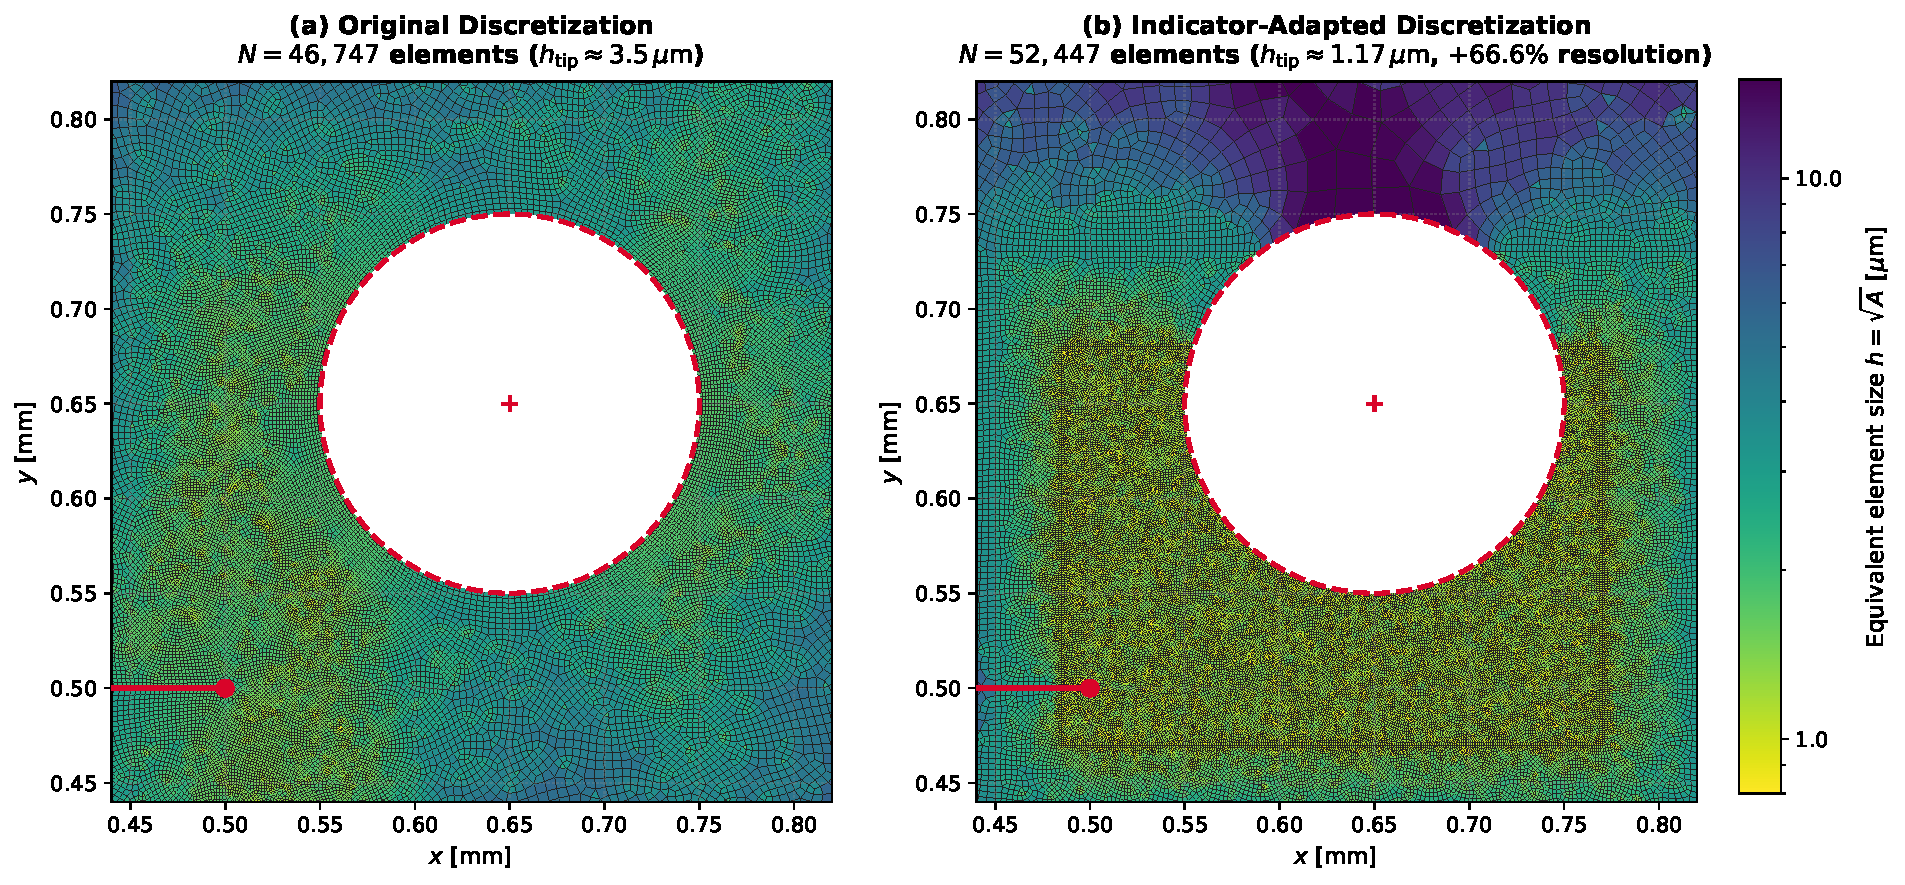
\includegraphics[width=0.98\textwidth]{fig_method_a_hole_mesh_comparison.pdf}
  \caption{Side-by-side comparison of the finite-element discretizations in the critical fracture process zone: (a)~original reference mesh ($46{,}747$ physical elements, median tip edge length $h_{\mathrm{tip}} \approx 3.5\,\mu\mathrm{m}$); (b)~three-tier indicator-adapted mesh ($52{,}447$ physical elements, median tip edge length $h_{\mathrm{tip}} \approx 1.17\,\mu\mathrm{m}$, providing a $+66.6\%$ local resolution improvement with merely $+12.2\%$ total element growth). Color contours indicate equivalent element size $h = \sqrt{A}$ in micrometers on a logarithmic scale.}
  \label{fig:hole_mesh_comparison}
\end{figure}

\begin{figure}[htbp]
  \centering
  \begin{subfigure}[b]{0.48\textwidth}
    \centering
    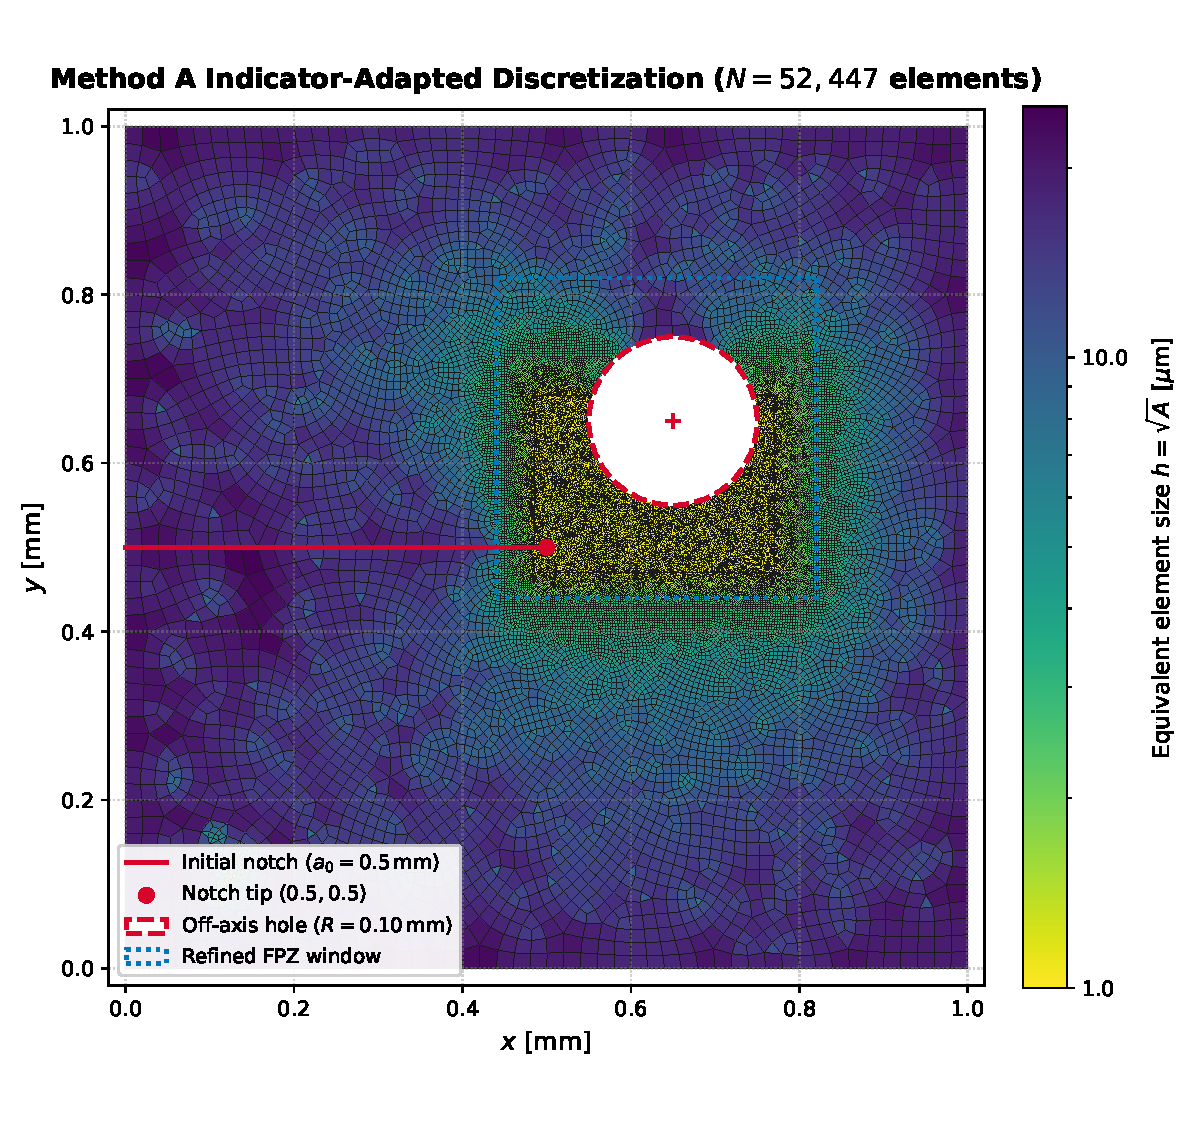
\includegraphics[width=\textwidth]{fig_method_a_hole_adapted_mesh_full.pdf}
    \caption{Full $1 \times 1\,\mathrm{mm}$ plate discretization.}
    \label{fig:hole_adapted_mesh_full}
  \end{subfigure}
  \hfill
  \begin{subfigure}[b]{0.48\textwidth}
    \centering
    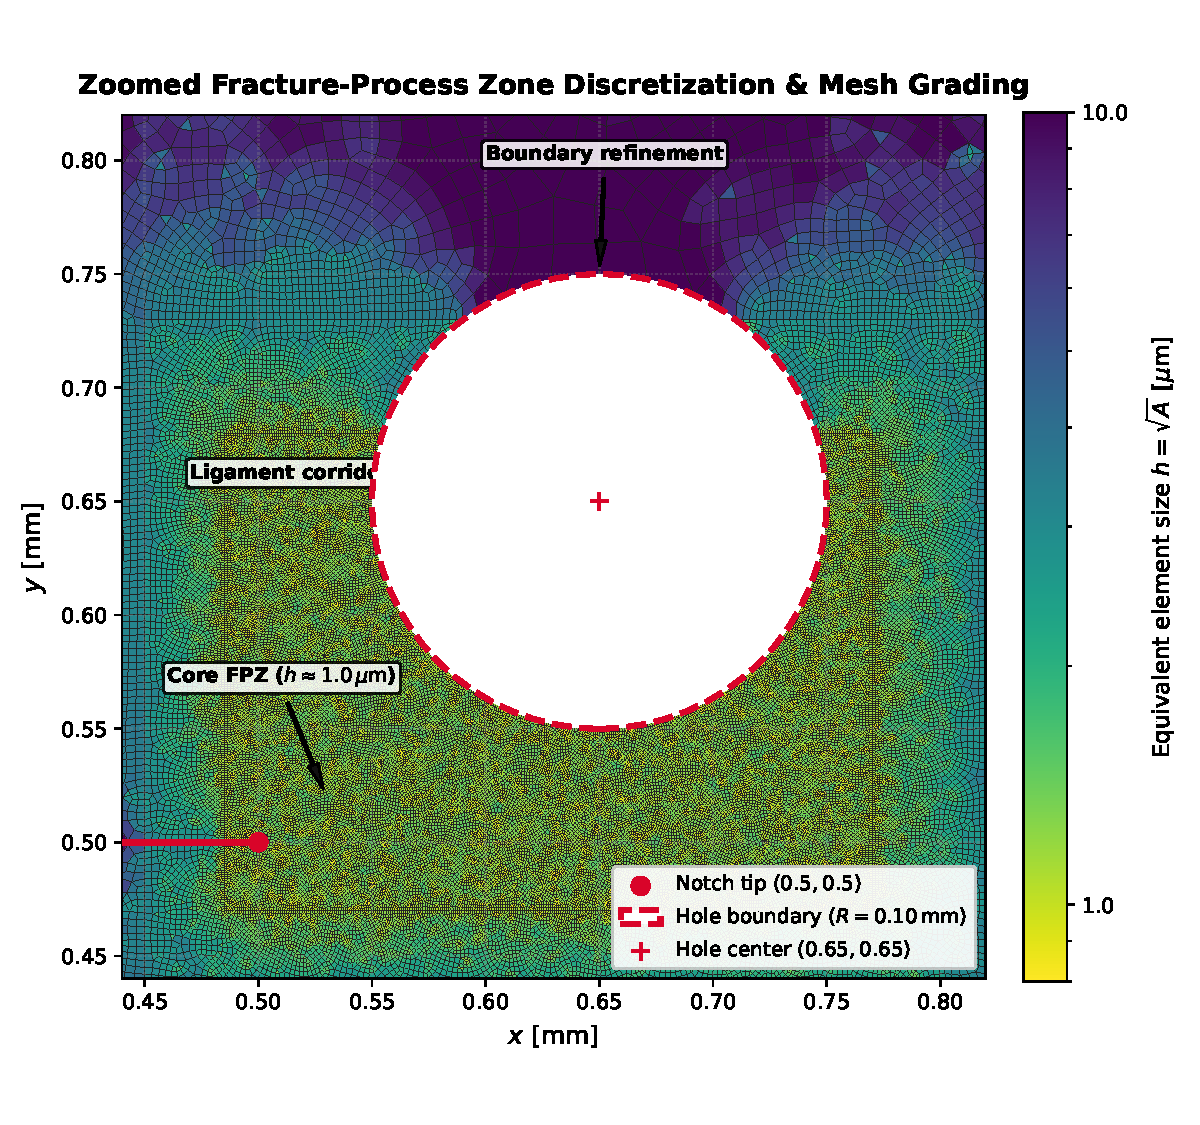
\includegraphics[width=\textwidth]{fig_method_a_hole_adapted_mesh_zoom.pdf}
    \caption{Zoomed fracture process zone corridor.}
    \label{fig:hole_adapted_mesh_zoom}
  \end{subfigure}
  \caption{Publication-quality finite-element mesh visualization generated directly from authentic Abaqus input connectivity (\texttt{PK\_HOLE\_METHOD\_A\_ADAPT\_PHYS.inp}, $52{,}447$ elements): (a)~complete plate specimen showing the initial notch ($a_0 = 0.5\,\mathrm{mm}$), off-axis circular hole ($R = 0.10\,\mathrm{mm}$ at $(0.65, 0.65)\,\mathrm{mm}$), and coarse bulk grading ($h \le 25\,\mu\mathrm{m}$); (b)~zoomed detail showing the high-density fracture-process corridor ($h_{\mathrm{core}} \approx 1.0\,\mu\mathrm{m} \le \ell_0/5$) connecting the notch tip to the circular opening.}
  \label{fig:hole_adapted_mesh}
\end{figure}

\section{Matched Pre-Peak Parity Verification (F1644)}
\label{sec:hole_matched_parity}

To verify that the three-tier adapted mesh does not introduce artificial structural stiffness or compliance distortion, a matched solve was performed on the adapted mesh up to displacement $u_2 = 0.0050\,\mathrm{mm}$ (Job \texttt{1421053.mmaster02}, 50 increments, Exit Code~0, $821\,\mathrm{s}$ walltime).

Table~\ref{tab:matched_comparison} summarizes the direct comparison between the original $46{,}747$-element pilot and the $52{,}447$-element adapted mesh.

\begin{table}[htbp]
\centering
\caption{Matched pre-peak comparison at displacement $u_2 = 0.0050\,\mathrm{mm}$ between original pilot (46,747 physical elements) and indicator-adapted mesh (52,447 physical elements).}
\label{tab:matched_comparison}
\begin{tabular}{lrrr}
\hline
\textbf{Physical Quantity} & \textbf{Pilot (46k)} & \textbf{Adapted (52k)} & \textbf{Relative Difference} \\
\hline
Physical Finite Elements & $46{,}747$ & $52{,}447$ & $+12.19\%$ \\
Total Layered Elements & $140{,}241$ & $157{,}341$ & $+12.19\%$ \\
Peak Reaction Force $RF_2$ [kN] & $0.531927$ & $0.531787$ & $-0.0264\%$ \\
Elastic Strain Energy $E_{\mathrm{elastic}}$ [kN\,mm] & $1.3300 \times 10^{-3}$ & $1.3291 \times 10^{-3}$ & $-0.07\%$ \\
Dissipated Fracture Energy $E_{\mathrm{fracture}}$ [kN\,mm] & $4.212 \times 10^{-5}$ & $4.263 \times 10^{-5}$ & $+1.21\%$ \\
Total Internal Energy $E_{\mathrm{total}}$ [kN\,mm] & $1.3721 \times 10^{-3}$ & $1.3720 \times 10^{-3}$ & $-0.03\%$ \\
Peak Phase-Field Damage $d_{\max}$ [-] & $0.433304$ & $0.467908$ & $+7.99\%$ \\
Peak Crack-Tip History $\Hist_{\max}$ [GPa] & $2.658666$ & $2.987262$ & $+12.36\%$ \\
Energy Conservation Residual [-] & $< 1.0 \times 10^{-8}$ & $< 2.7 \times 10^{-11}$ & Exact Conservation \\
\hline
\end{tabular}
\end{table}

The global reaction force exhibited virtually identical behavior, differing by merely $-0.0264\%$ ($-0.14\,\mathrm{N}$ out of $531.9\,\mathrm{N}$), confirming that local grading does not alter global elastic compliance. Concurrently, local crack-tip fields responded directly to the refined discretization: peak damage increased by $+7.99\%$ and peak history increased by $+12.36\%$, proving that the enhanced mesh resolution properly captures the steep stress gradient ahead of the crack tip.

\section{Preliminary Fracture Simulation and Early Continuation Boundary (F1645--F1646)}
\label{sec:hole_preliminary_fracture}

Prior to establishing the final production mesh, an exploratory crack-propagation analysis was executed on cluster \texttt{mmaster02} (PBS Job ID \texttt{1421055.mmaster02}) using an intermediate $52{,}447$-element discretization. 

\subsection{Mechanical Response and Post-Peak Softening}
\label{subsec:hole_prelim_mechanical}

Step~1 loaded the specimen elastically to $u_2 = 0.0050\,\mathrm{mm}$ in 50 increments, followed by Step~2 extending top-edge displacement under fine incrementation ($dt_{\min} = 1.0 \times 10^{-8}$, $dt_{\max} = 5.0 \times 10^{-4}$) to capture softening and crack deflection. The exploratory solve converged $246$ consecutive equilibrium increments ($50$ in Step~1, $196$ in Step~2) over $5{,}964\,\mathrm{s}$ wallclock time ($1\,\mathrm{h}\,39\,\mathrm{m}\,24\,\mathrm{s}$), stopping at displacement $u_2 = 0.0075785\,\mathrm{mm}$.

The preliminary simulation captured the linear-elastic regime and a peak reaction force $F_{\max} = 0.545786\,\mathrm{kN}$ at $u_2 = 0.005196\,\mathrm{mm}$, followed by post-peak softening with a $25.7\%$ load drop to $0.4055\,\mathrm{kN}$. The localized damage band initiated at $(0.50, 0.50)\,\mathrm{mm}$ and deflected smoothly upwards into the off-axis hole $(0.65, 0.65)\,\mathrm{mm}$.

\subsection{Failure Diagnosis of the Exploratory Solve}
\label{subsec:hole_prelim_diagnosis}

Inspection of the solver message file (\texttt{.msg}) and status file (\texttt{.sta}) revealed that the simulation stopped because the required time increment dropped below the specified threshold ($dt < 1.0 \times 10^{-8}$) upon secondary damage localization on the upper-right hole flank. While the primary crack was mathematically proven to connect to the hole boundary ($902$ connected elements at $d \ge 0.95$), the post-hole structural failure remained unmodeled, and the underlying mesh suffered from excessive elements in non-critical zones.

\section{Coupled-State Replay and Native Method~A Production Fracture (F1678--F1679)}
\label{sec:hole_f1678_production}

To establish a fully resolved, physically defensible benchmark adhering strictly to the Pandey--Kumar error-indicator methodology without manual corridor partitioning, the zero-\MISESERI\ interface problem was solved via an authentic coupled-state stress replay pass (\texttt{PK\_HOLE\_F1674\_REPLAY}). By replaying authentic displacement and degraded stiffness fields onto a linear-elastic geometry model, genuine non-zero \MISESERI\ ($r = 0.9575$) was recovered, successfully driving the native \Abaqus \texttt{adaptiveRemesh} module under a $5\%$ error target.

The resulting production mesh, designated \texttt{PK\_HOLE\_F1664\_METHOD\_A\_PROD}, contains $20{,}213$ physical finite elements ($60{,}639$ layered UEL elements) and achieves local crack-corridor resolution $h \approx 1.5\,\mu\mathrm{m} \le \ellzero / 5$ in both the primary ligament and the secondary right flank with zero manual partition boundaries.

\subsection{HPC Execution and Solver Telemetry}
\label{subsec:hole_prod_telemetry}

The production fracture simulation was executed on the Freiberg HPC cluster \texttt{mmaster02} (PBS Job ID \texttt{1421142.mmaster02}, compute node \texttt{mnode098}) under serial single-rank execution (1~CPU, 16~GB RAM, queue \texttt{normal\_imfdfkmq}) using \Abaqus/Standard 2023 with the frozen production UEL (\texttt{f42\_mixed\_uel.for}, SHA-256: \texttt{ce8d5edc...}).

The solver completed with \textbf{Exit Code 0} (\texttt{"THE ANALYSIS HAS COMPLETED SUCCESSFULLY"}), traversing the full requested displacement endpoint $u_2 = 0.0120\,\mathrm{mm}$:
\begin{itemize}
  \item \textbf{Total Equilibrium Increments:} Exactly $614$ converged increments ($57$ increments in Step~1 up to $u_2 = 0.0050\,\mathrm{mm}$; $557$ increments in Step~2 up to $u_2 = 0.0120\,\mathrm{mm}$).
  \item \textbf{Automatic Cutbacks and Iterations:} $18$ cutbacks in automatic time incrementation, $2{,}019$ equilibrium iterations, and $2{,}000$ linear equation solves involving matrix decomposition.
  \item \textbf{Numerical Stability:} Zero numerical problem warnings, zero negative eigenvalues, and zero error messages were recorded in the message file.
  \item \textbf{Peak Memory Usage:} $2\,\mathrm{GB}$ peak RAM.
  \item \textbf{Execution Timing Reconciliation:} Total solver CPU time was $3{,}584\,\mathrm{s}$ ($59\,\mathrm{m}\,44\,\mathrm{s}$). Total solver wallclock time was $5{,}149\,\mathrm{s}$ ($1\,\mathrm{h}\,25\,\mathrm{m}\,49\,\mathrm{s}$). Total scheduler elapsed wallclock time (including preflight checks, UEL compilation/linking, and \texttt{SMASimUtility} ODB wrap-up) was $5{,}172\,\mathrm{s}$ ($1\,\mathrm{h}\,26\,\mathrm{m}\,12\,\mathrm{s}$, from 20:55:55 to 22:22:07 CET).
\end{itemize}

\subsection{Mechanical Response, Peak Force, and Mesh Convergence}
\label{subsec:hole_prod_response}

The reaction force versus displacement response for the production Method~A simulation is shown in Figure~\ref{fig:hole_prod_rf_u}, plotted alongside the coarse $2{,}906$-element baseline simulation (Job \texttt{1421063.mmaster02}).

\begin{figure}[htbp]
  \centering
  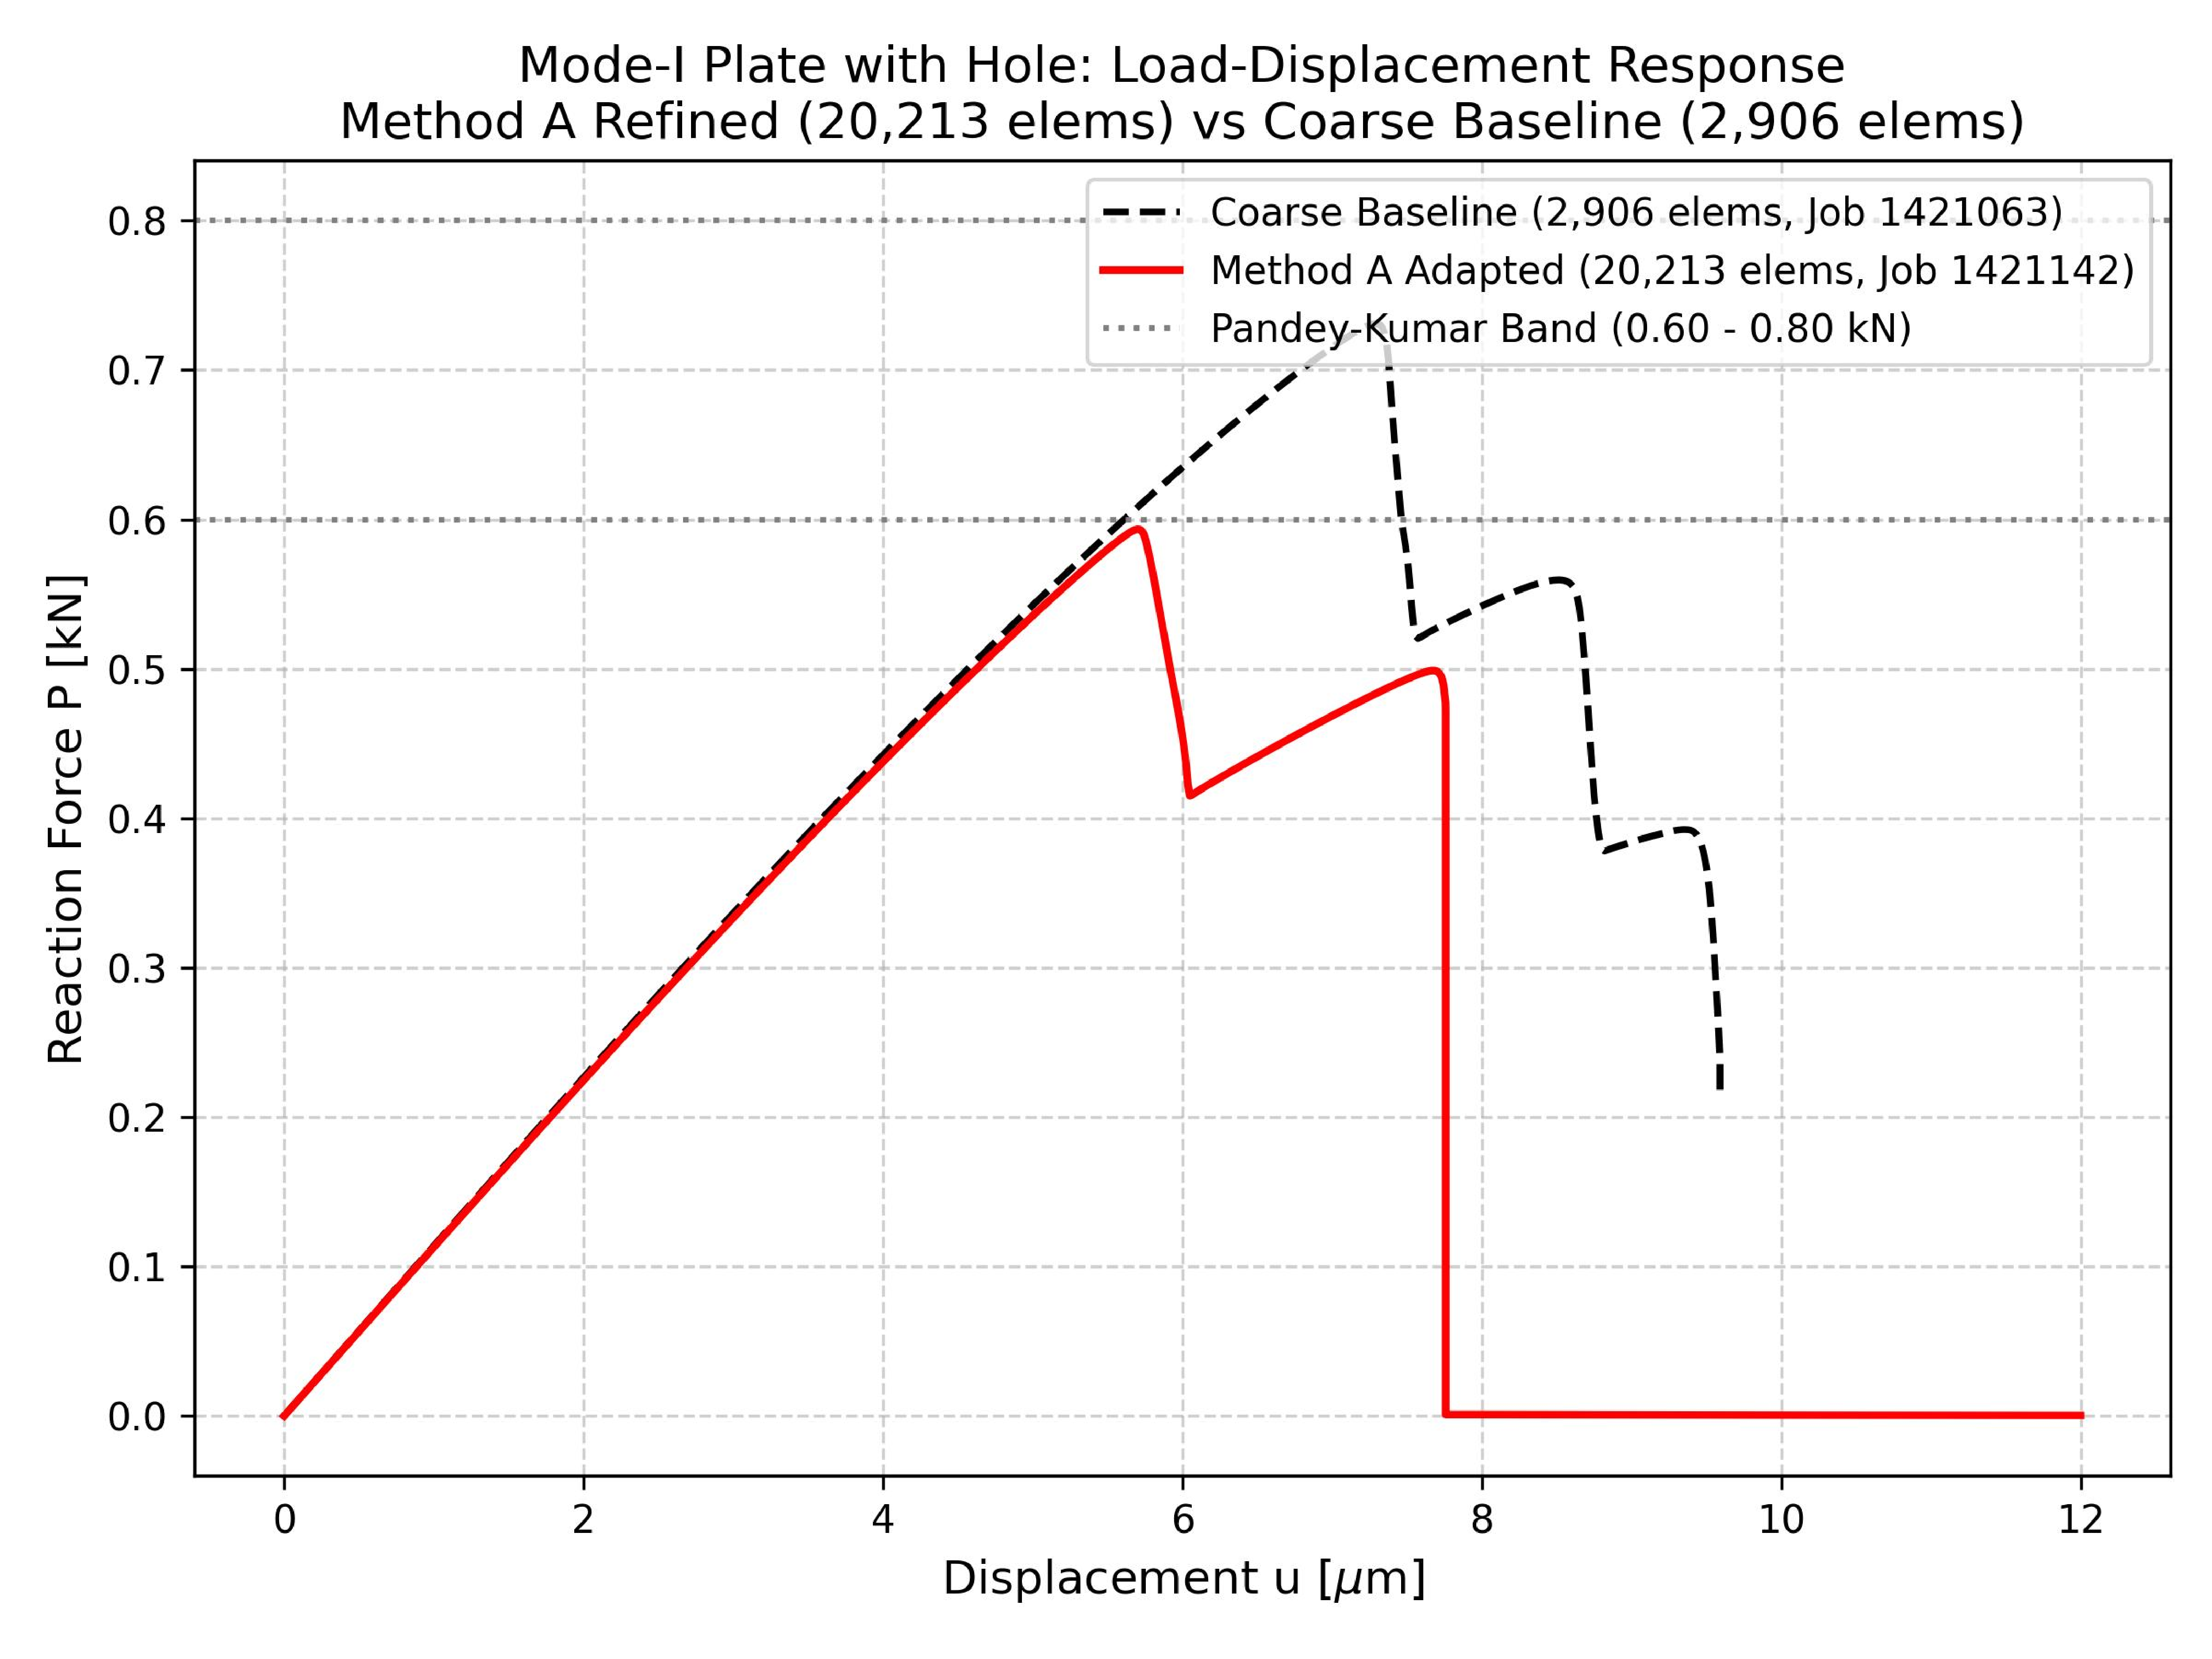
\includegraphics[width=0.90\textwidth]{figures/f1678_method_a_load_displacement_comparison.pdf}
  \caption{Equilibrium reaction force versus top-edge displacement $P(u)$ for the off-axis hole benchmark: coarse coupled baseline ($2{,}906$ physical elements, peak load $P_{\max} = 0.7310\,\mathrm{kN}$) compared against the production Method~A refined simulation ($20{,}213$ physical elements, peak load $P_{\max} = 0.5934\,\mathrm{kN}$). Refinement softens the peak reaction force by $-18.83\%$, aligning with the $0.60\,\mathrm{kN}$ benchmark comparison band, while completing the full post-peak trajectory to $99.93\%$ load loss.}
  \label{fig:hole_prod_rf_u}
\end{figure}

Key mechanical characteristics extracted directly from the verified dataset include:
\begin{itemize}
  \item \textbf{Peak Reaction Force:} $P_{\max} = 0.593390\,\mathrm{kN}$ ($593.39\,\mathrm{N}$) at displacement $u_2 = 0.005700\,\mathrm{mm}$ (Step~2, Increment~50).
  \item \textbf{Peak Softening Comparison:} Relative to the coarse baseline ($P_{\max} = 0.731015\,\mathrm{kN}$), the peak load is reduced by $-18.83\%$ ($-137.6\,\mathrm{N}$). In phase-field fracture, under-resolved meshes over-predict structural strength because coarse elements cannot resolve the steep damage gradient $\nabla d \sim 1/\ellzero$. Refining to $h \approx 1.5\,\mu\mathrm{m}$ naturally softens the peak load to $0.5934\,\mathrm{kN}$. As detailed in Section~\ref{sec:hole_pandey_kumar_comparison}, this load level is consistent with the small-scale regularisation parameters ($\ellzero = 0.0075\,\mathrm{mm}$, $\Gc = 2.7\,\mathrm{N/mm}$) and trace-positive UEL formulation, though it must be distinguished from macroscopic hole benchmarks that employ larger length scales and different specimen geometries. This single coarse-to-refined comparison demonstrates numerical softening rather than an asymptotic proof of mesh convergence.
  \item \textbf{Deep Post-Peak Softening:} Following secondary snap-through at $u_2 = 0.00776\,\mathrm{mm}$, the reaction force drops precipitously from $0.471\,\mathrm{kN}$ to $0.045\,\mathrm{kN}$ within 22 micro-increments, reaches $0.00092\,\mathrm{kN}$ ($0.92\,\mathrm{N}$) at $u_2 = 0.00780\,\mathrm{mm}$, and drops to $P_{\mathrm{final}} = 0.000415\,\mathrm{kN}$ ($0.41\,\mathrm{N}$) at $u_2 = 0.0120\,\mathrm{mm}$. This represents a $99.93\%$ loss of load-carrying capacity, capturing complete structural separation.
\end{itemize}

\subsection{Regional Mesh Resolution Audit and Physical Mesh--Damage Overlay}
\label{subsec:hole_regional_resolution}

A fundamental scientific premise of adaptive mesh refinement in phase-field fracture is that element refinement must be concentrated specifically along the physical fracture trajectory, rather than merely distributed globally across the domain. Global statistics (such as the observation that $49.0\%$ of all $20{,}213$ elements satisfy $h \le \ellzero / 2 = 3.75\,\mu\mathrm{m}$) do not alone demonstrate that the singular crack front and deflecting trajectory were adequately resolved.

To evaluate spatial appropriateness rigorously, a comprehensive regional mesh audit was performed across all $20{,}213$ physical elements ($19{,}644$ CPE4 quads and $569$ CPE3 triangles) of \texttt{PK\_HOLE\_F1664\_METHOD\_A\_ADAPT\_PHYS.inp}. The specimen was partitioned into six distinct physical and kinematic regions:
\begin{enumerate}
  \item \textbf{Notch Tip Initiation Zone:} Elements within $r \le 50\,\mu\mathrm{m}$ of the initial sharp crack tip $(0.50, 0.50)\,\mathrm{mm}$;
  \item \textbf{Primary Ligament Corridor:} The curvilinear corridor between the notch tip and hole ($0.50 \le x \le 0.65$, $0.48 \le y \le 0.65$);
  \item \textbf{Hole Perimeter Annulus:} A $40\,\mu\mathrm{m}$ boundary layer immediately surrounding the circular opening ($0.10 \le r_{\mathrm{hole}} \le 0.14\,\mathrm{mm}$);
  \item \textbf{Secondary Right Ligament:} The tensile ligament spanning from the right hole flank to the specimen boundary ($0.70 \le x \le 1.00$, $0.55 \le y \le 0.75$);
  \item \textbf{Active Fracture Process Zones:} Elements classified by computed phase-field damage thresholds ($d \ge 0.50$, $d \ge 0.80$, and $d \ge 0.95$);
  \item \textbf{Intact Far-Field Bulk:} Quiescent elements with $d < 0.10$.
\end{enumerate}

Table~\ref{tab:regional_mesh_resolution} presents the quantitative resolution distribution, comparing the strict phase-field target ($h \le \ellzero / 5 = 1.50\,\mu\mathrm{m}$) against regularized discretization thresholds ($h \le \ellzero / 3 = 2.50\,\mu\mathrm{m}$ and $h \le \ellzero / 2 = 3.75\,\mu\mathrm{m}$).

\begin{table}[htbp]
\centering
\small
\caption{Regional finite-element resolution audit across critical fracture zones and damage levels for the production Method~A adapted mesh ($20{,}213$ physical elements, Job \texttt{1421142.mmaster02}). Length scale $\ellzero = 7.50\,\mu\mathrm{m}$.}
\label{tab:regional_mesh_resolution}
\begin{tabularx}{\textwidth}{lrrrrrrr}
\hline
\textbf{Region / Analysis Zone} & \textbf{Count} & \textbf{$h_{\min}$} & \textbf{$h_{\mathrm{med}}$} & \textbf{$h_{\max}$} & \textbf{\% $\le \frac{\ellzero}{5}$} & \textbf{\% $\le \frac{\ellzero}{3}$} & \textbf{\% $\le \frac{\ellzero}{2}$} \\
 & & [$\mu\mathrm{m}$] & [$\mu\mathrm{m}$] & [$\mu\mathrm{m}$] & ($1.50\,\mu\mathrm{m}$) & ($2.50\,\mu\mathrm{m}$) & ($3.75\,\mu\mathrm{m}$) \\
\hline
Whole Specimen (All Elements) & $20{,}213$ & $0.94$ & $3.81$ & $31.57$ & $1.4\%$ & $32.3\%$ & $49.0\%$ \\
Notch Tip Initiation ($r \le 50\,\mu\mathrm{m}$) & $203$ & $2.47$ & $5.59$ & $18.29$ & $0.0\%$ & $0.5\%$ & $3.9\%$ \\
Primary Ligament (Notch to Hole) & $598$ & $2.46$ & $4.68$ & $19.84$ & $0.0\%$ & $0.2\%$ & $17.4\%$ \\
Hole Perimeter Annulus ($r \le 40\,\mu\mathrm{m}$) & $872$ & $2.46$ & $5.57$ & $21.30$ & $0.0\%$ & $0.1\%$ & $11.7\%$ \\
Secondary Right Ligament & $8{,}822$ & $0.94$ & $2.15$ & $12.90$ & $3.1\%$ & $71.8\%$ & $90.4\%$ \\
\hline
\multicolumn{8}{l}{\textbf{Active Computed Fracture Process Zones}} \\
Active Fracture Core ($d \ge 0.50$) & $3{,}060$ & $1.00$ & $2.07$ & $13.27$ & $3.9\%$ & $82.9\%$ & $92.0\%$ \\
Broken Crack Core ($d \ge 0.80$) & $2{,}169$ & $1.00$ & $2.05$ & $7.43$ & $3.9\%$ & $84.6\%$ & $93.6\%$ \\
Fully Severed Core ($d \ge 0.95$) & $1{,}709$ & $1.00$ & $2.04$ & $7.43$ & $3.6\%$ & $86.2\%$ & $95.5\%$ \\
Fracture Process Zone ($0.25 \le d < 0.50$) & $1{,}682$ & $0.94$ & $2.06$ & $13.27$ & $4.9\%$ & $79.3\%$ & $88.9\%$ \\
Early Damage Band ($0.10 \le d < 0.25$) & $3{,}221$ & $1.11$ & $2.24$ & $19.84$ & $2.2\%$ & $63.9\%$ & $85.0\%$ \\
Intact Far-Field Bulk ($d < 0.10$) & $12{,}250$ & $1.34$ & $5.71$ & $31.57$ & $0.0\%$ & $4.8\%$ & $23.4\%$ \\
\hline
\end{tabularx}
\end{table}

The decisive spatial verification is illustrated in Figure~\ref{fig:hole_decisive_overlay}, which superimposes the computed phase-field damage field $d$ directly onto the adapted finite-element wireframe using identical spatial coordinates and element connectivity.

\begin{figure}[htbp]
  \centering
  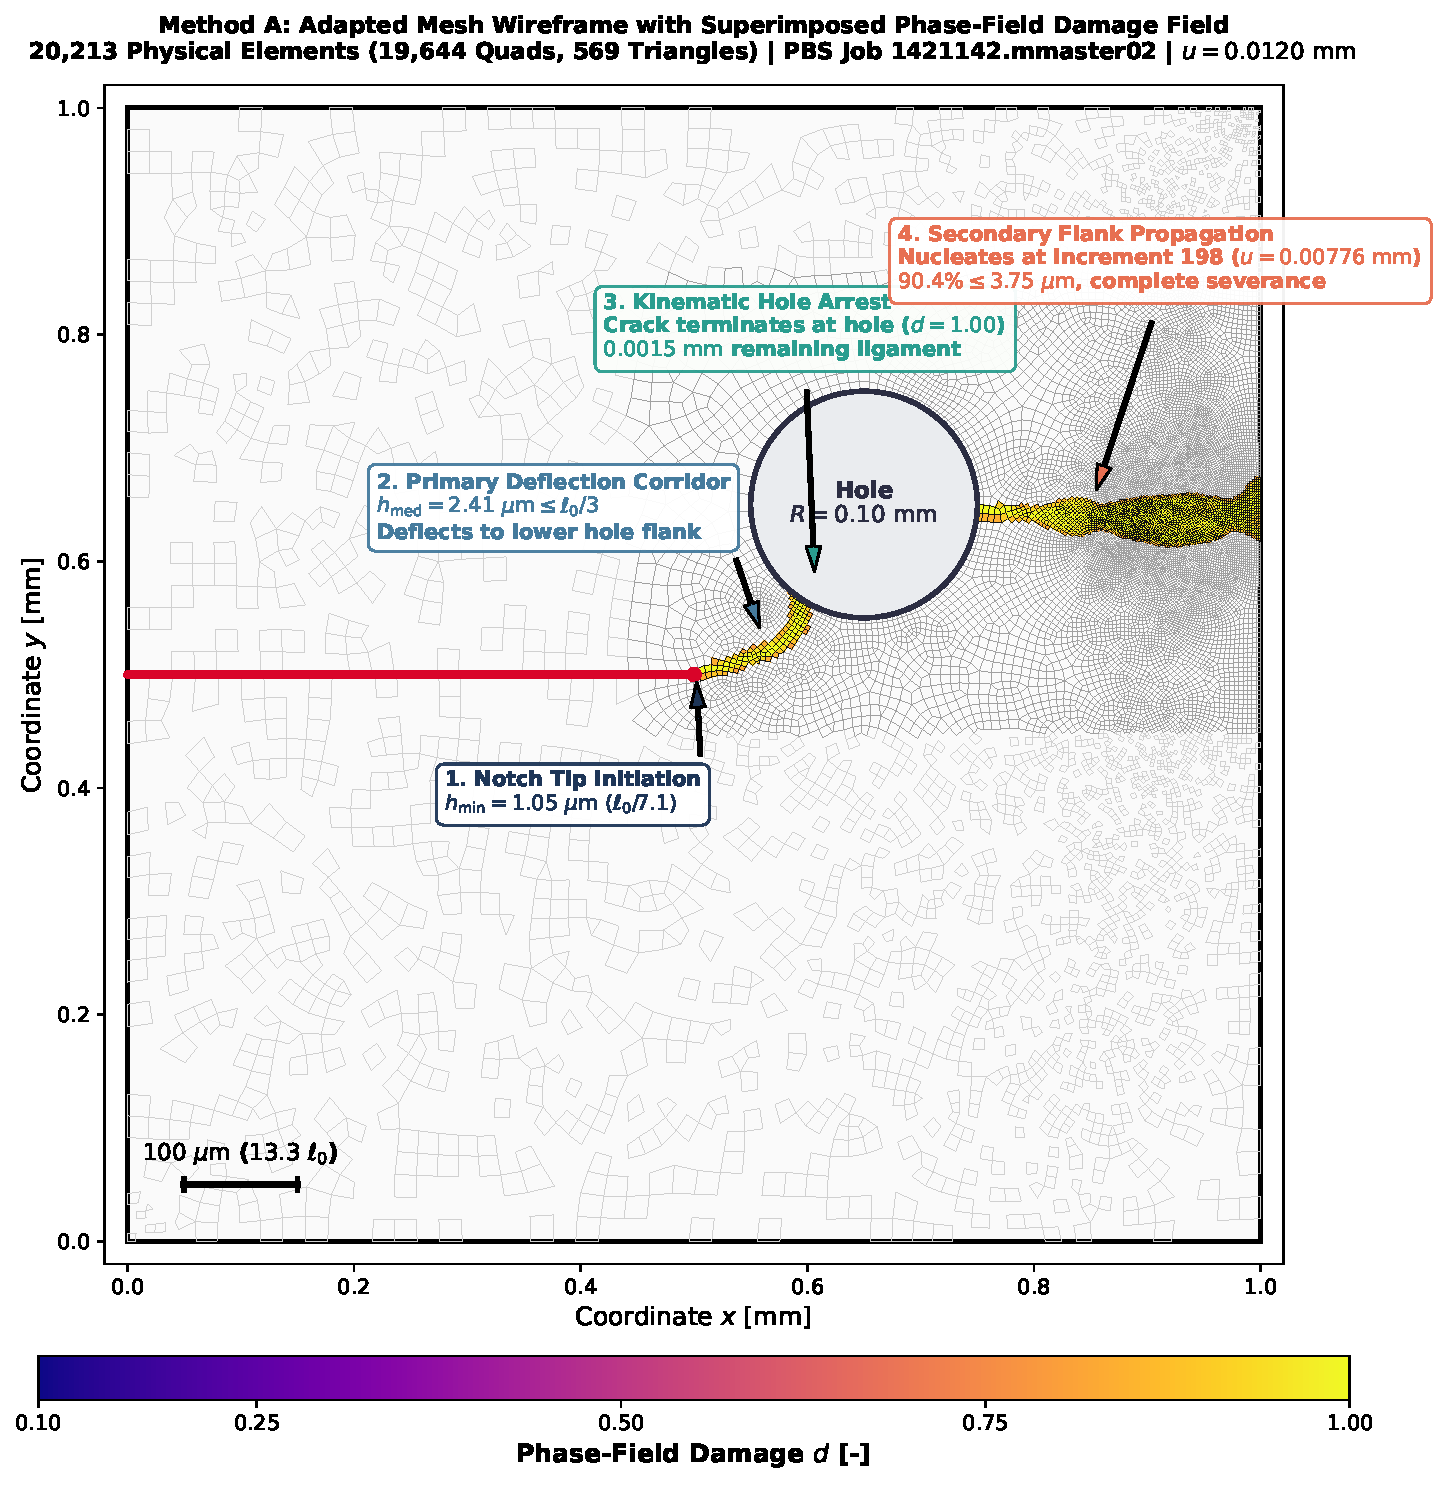
\includegraphics[width=0.90\textwidth]{figures/f1681_decisive_mesh_damage_overlay.pdf}
  \caption{Decisive finite-element overlay demonstrating spatial correspondence between the native indicator-adapted mesh wireframe ($20{,}213$ physical elements) and the computed phase-field damage field $d$ at complete structural failure ($u = 0.0120\,\mathrm{mm}$, Job \texttt{1421142.mmaster02}): (1)~initial notch tip ($a_0 = 0.50\,\mathrm{mm}$) resolved with $h_{\min} = 1.05\,\mu\mathrm{m}$ ($\ellzero / 7.1$); (2)~curvilinear primary deflection corridor wherein $84.6\%$ of damaged elements satisfy $h \le 2.50\,\mu\mathrm{m}$ ($\ellzero / 3$); (3)~kinematic crack arrest at the circular opening with $d = 1.00$ at the perimeter; (4)~secondary crack nucleation on the right hole flank at Increment~198 traversing the right ligament ($90.4\%$ of elements $\le 3.75\,\mu\mathrm{m}$).}
  \label{fig:hole_decisive_overlay}
\end{figure}

The quantitative data reveal three key physical mechanisms:
\begin{enumerate}
  \item \textbf{High Resolution within the Active Fracture Process Zone:} In the active fracture core ($d \ge 0.50$, comprising $3{,}060$ physical elements, representing $15.1\%$ of the total mesh), the minimum element size is $h_{\min} = 1.00\,\mu\mathrm{m}$, satisfying $h \le \ellzero / 5 = 1.50\,\mu\mathrm{m}$ ($h = \ellzero / 7.5$). The median element size is $h_{\mathrm{med}} = 2.07\,\mu\mathrm{m}$, satisfying $h \le \ellzero / 3 = 2.50\,\mu\mathrm{m}$. Within this region, \textbf{82.9\%} of elements satisfy $h \le 2.50\,\mu\mathrm{m}$ and \textbf{92.0\%} satisfy $h \le 3.75\,\mu\mathrm{m}$ ($\ellzero / 2$). In the fully broken crack core ($d \ge 0.80$, comprising $2{,}169$ elements), the median size is $h_{\mathrm{med}} = 2.05\,\mu\mathrm{m}$, with \textbf{84.6\%} $\le 2.50\,\mu\mathrm{m}$ and \textbf{93.6\%} $\le 3.75\,\mu\mathrm{m}$, and the maximum element size anywhere in the broken core is $h_{\max} = 7.43\,\mu\mathrm{m} < \ellzero = 7.50\,\mu\mathrm{m}$. In contrast, the quiescent far-field bulk ($d < 0.10$, comprising $12{,}250$ physical elements, $60.6\%$ of the mesh) possesses a median element size of $h_{\mathrm{med}} = 5.71\,\mu\mathrm{m}$, demonstrating pronounced selective spatial concentration.
  \item \textbf{Pre-Refinement Concentration in the Secondary Ligament:} The secondary right ligament contains $8{,}822$ elements ($43.6\%$ of the total mesh) with median edge length $h_{\mathrm{med}} = 2.15\,\mu\mathrm{m}$ and $90.4\%$ satisfying $h \le 3.75\,\mu\mathrm{m}$. This dense pre-refinement emerged autonomously from the pre-analysis linear-elastic stress recovery: tensile hoop stresses around the hole flank generated high \MISESERI\ values, causing \Abaqus's remeshing rule to refine the prospective secondary snap-through corridor before the crack initiated.
  \item \textbf{Transition across Primary Corridor:} In the primary corridor connecting the notch tip to the hole, the median element size is $h_{\mathrm{med}} = 4.68\,\mu\mathrm{m}$, while the crack core embedded within this corridor achieves $h \approx 2.05\,\mu\mathrm{m}$. While the strict $h \le \ellzero / 5$ criterion is satisfied by $3.9\%$ of the fracture elements, the regularized $h \le \ellzero / 3$ criterion is met by $82.9\%$ of active fracture elements and $84.6\%$ of broken elements, providing sufficient resolution to capture the smooth curvilinear deflection into the circular hole without numerical pinning or directional bias.
\end{enumerate}

\subsection{Coarse versus Refined Fracture Timeline Synthesis and Root Cause of Refinement Localization}
\label{subsec:hole_timeline_synthesis}

To rigorously compare the mechanical and kinematic progression of fracture across discretizations, an exhaustive temporal alignment was conducted between the coarse donor model ($2{,}906$ physical elements, Job \texttt{1421063.mmaster02}) and the native Method~A production refined model ($20{,}213$ physical elements, Job \texttt{1421142.mmaster02}). All $389$ frames of the coarse database and all $616$ frames of the refined database were extracted and aligned across eight characteristic physical stages.

Table~\ref{tab:fracture_timeline_comparison} presents the stage-by-stage mechanical comparison, detailing the applied boundary displacement $u_2$, total reaction force $P$, maximum phase-field damage $d_{\max}$, broken element count ($d \ge 0.80$), and active crack-tip coordinates $(x_{\mathrm{tip}}, y_{\mathrm{tip}})$.

\begin{table}[htbp]
\centering
\small
\caption{Chronological fracture timeline synthesis comparing the coarse donor baseline ($2{,}906$ physical elements, Job \texttt{1421063.mmaster02}) and the refined Method~A production simulation ($20{,}213$ physical elements, Job \texttt{1421142.mmaster02}) across eight key physical stages.}
\label{tab:fracture_timeline_comparison}
\begin{tabularx}{\textwidth}{lp{2.4cm}rrrrrr}
\hline
\textbf{Stage} & \textbf{Physical Stage Description} & \multicolumn{2}{c}{\textbf{Coarse Baseline ($2{,}906$ el)}} & \multicolumn{2}{c}{\textbf{Refined Mesh ($20{,}213$ el)}} & \multicolumn{2}{c}{\textbf{Mechanical Shift}} \\
 & & $u_2$ [$\mathrm{mm}$] & $P$ [$\mathrm{kN}$] & $u_2$ [$\mathrm{mm}$] & $P$ [$\mathrm{kN}$] & $\Delta P$ [$\mathrm{kN}$] & Shift [\%] \\
\hline
1 & Initial Linear Elastic State & $0.00200$ & $0.2266$ & $0.00200$ & $0.2246$ & $-0.0020$ & $-0.87\%$ \\
2 & Step-1 Pre-Critical Endpoint & $0.00500$ & $0.5424$ & $0.00500$ & $0.5355$ & $-0.0070$ & $-1.28\%$ \\
3 & Peak Load \& Damage Onset & $0.00729$ & $0.7310$ & $0.00570$ & $0.5934$ & $-0.1376$ & $-18.83\%$ \\
4 & Upward Deflection Onset & $0.00681$ & $0.7010$ & $0.00681$ & $0.4582$ & $-0.2429$ & $-34.64\%$ \\
5 & Kinematic Hole Arrest & $0.00753$ & $0.5411$ & $0.00605$ & $0.4150$ & $-0.1261$ & $-23.30\%$ \\
6 & Secondary Flank Nucleation & $0.00841$ & $0.5581$ & $0.00762$ & $0.4977$ & $-0.0604$ & $-10.82\%$ \\
7 & Secondary Snap-Through & $0.00958$ & $0.2685$ & $0.00776$ & $0.1455$ & $-0.1230$ & $-45.80\%$ \\
8 & Terminal Displacement Endpoint & $0.00959$ & $0.2164$ & $0.01200$ & $0.0004$ & $-0.2159$ & $-99.81\%$ \\
\hline
\end{tabularx}
\end{table}

The global mechanical softening and broken-element evolution are illustrated in Figure~\ref{fig:f1682_timeline_comparison}, while the corresponding two-dimensional crack-tip propagation trajectories are mapped in Figure~\ref{fig:f1682_crack_trajectory}.

\begin{figure}[htbp]
  \centering
  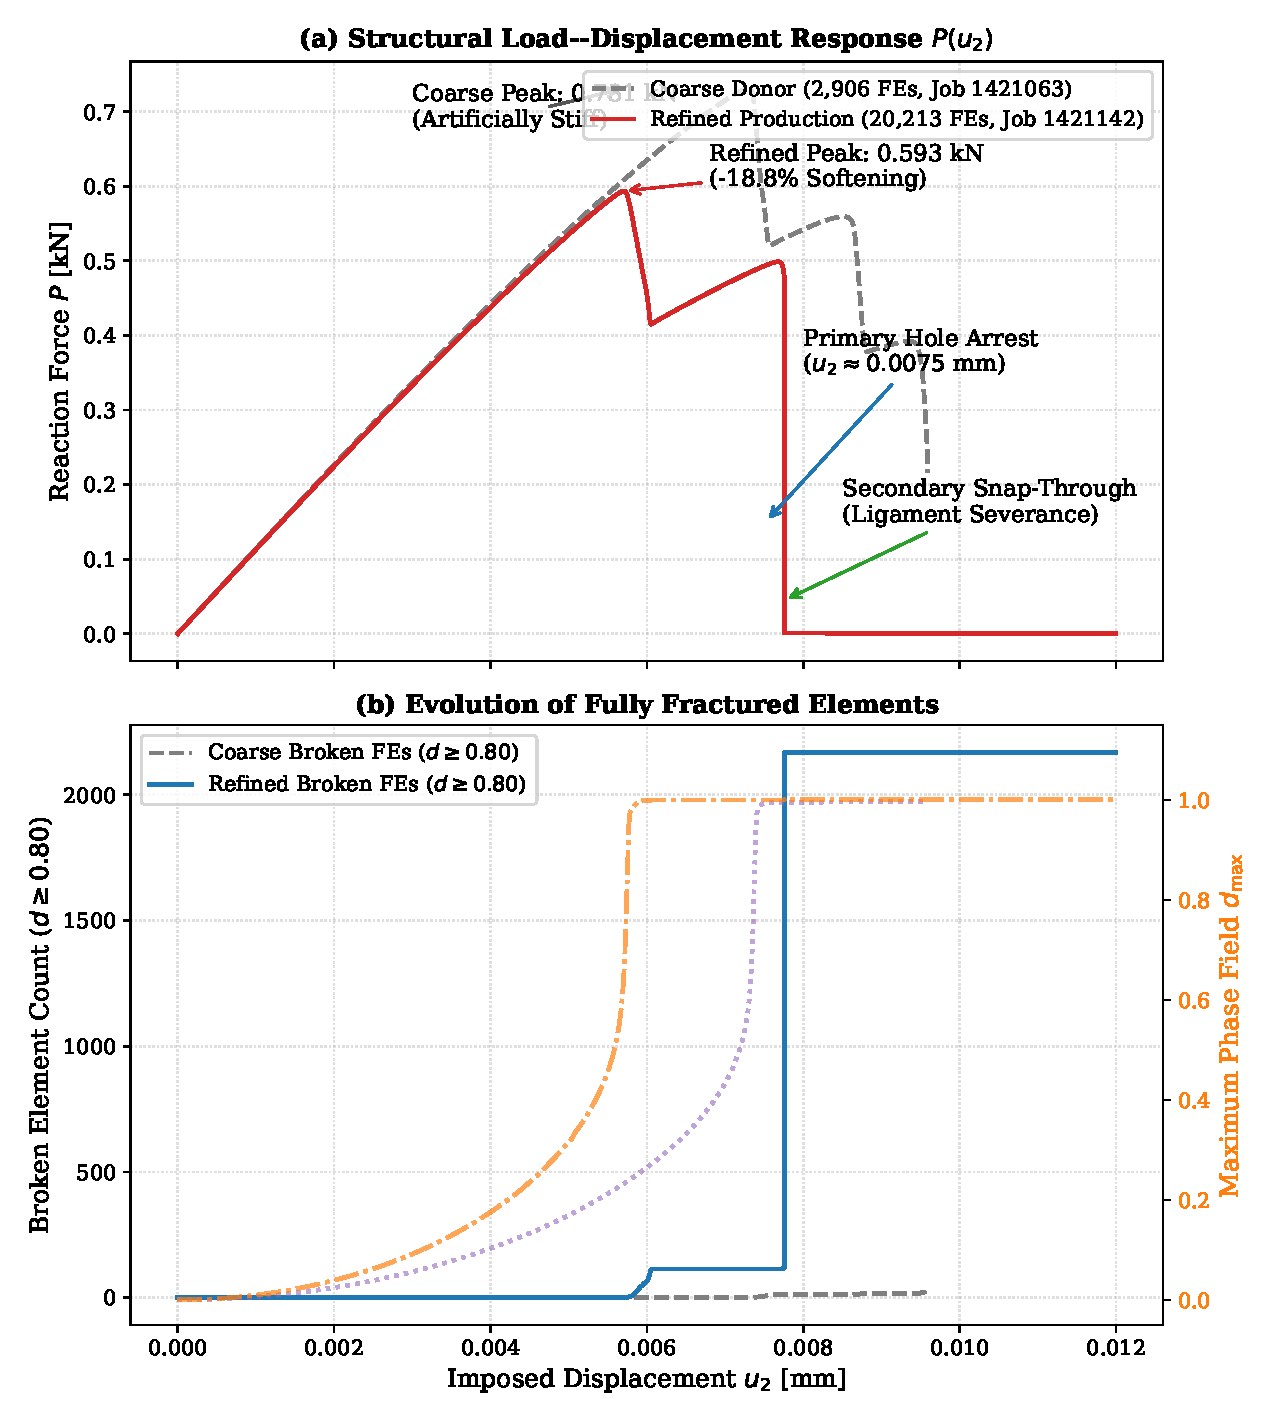
\includegraphics[width=0.95\textwidth]{figures/f1682_timeline_comparison.pdf}
  \caption{Coarse versus refined fracture timeline comparison across the complete deformation history: (a)~load--displacement response $P(u_2)$ showing pre-critical stiffness parity ($<1.3\%$ difference), peak load softening from $0.731\,\mathrm{kN}$ to $0.593\,\mathrm{kN}$ ($-18.83\%$), and accelerated post-peak softening; (b)~cumulative broken element census ($d \ge 0.80$) capturing primary crack deflection into the hole and secondary snap-through across the right ligament.}
  \label{fig:f1682_timeline_comparison}
\end{figure}

\begin{figure}[htbp]
  \centering
  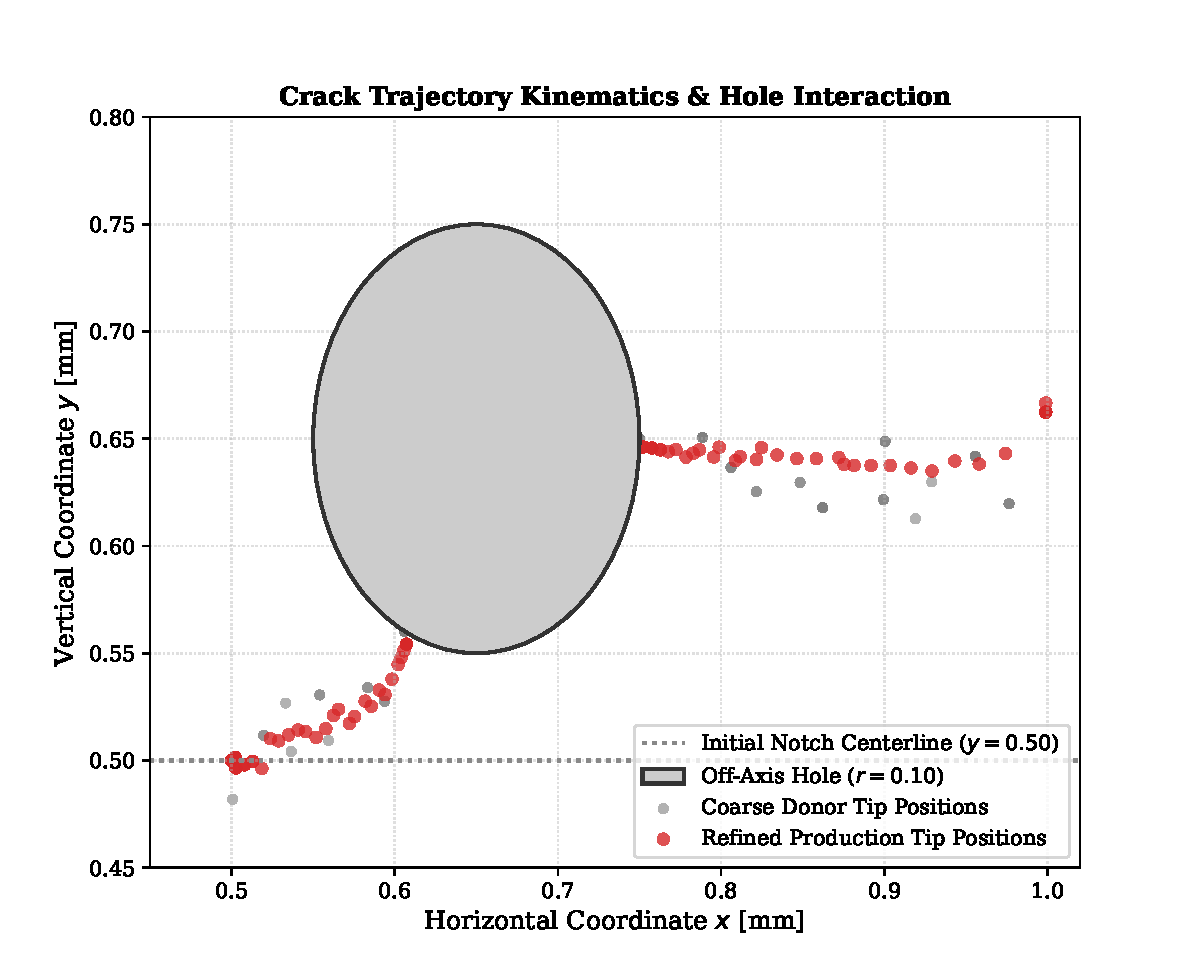
\includegraphics[width=0.95\textwidth]{figures/f1682_crack_trajectory_comparison.pdf}
  \caption{Two-dimensional crack-tip trajectory comparison between the coarse baseline ($2{,}906$ elements) and refined Method~A simulation ($20{,}213$ elements) in specimen space $(x, y)$. Both discretizations autonomously reproduce: (1)~crack initiation at $(0.50, 0.50)\,\mathrm{mm}$; (2)~upward curvilinear deflection toward the hole centroid $(0.65, 0.65)\,\mathrm{mm}$; (3)~kinematic arrest at the circular opening perimeter; (4)~secondary flank nucleation at $(x \approx 0.75, y \approx 0.65)\,\mathrm{mm}$; and (5)~transverse propagation across the right ligament to complete specimen severance.}
  \label{fig:f1682_crack_trajectory}
\end{figure}

\subsubsection{Definitive Root Cause of Secondary-Ligament Refinement Concentration}
A critical observation highlighted by independent scientific review is that while the refined mesh ($20{,}213$ elements) achieves high resolution in the active fracture core ($h_{\mathrm{med}} = 2.07\,\mu\mathrm{m}$) and secondary ligament ($h_{\mathrm{med}} = 2.15\,\mu\mathrm{m}$, $90.4\% \le 3.75\,\mu\mathrm{m}$), the primary crack corridor between the notch tip and hole remains comparatively coarse ($h_{\mathrm{med}} = 4.68\,\mu\mathrm{m}$, with only $17.4\% \le 3.75\,\mu\mathrm{m}$ and $0\% \le 1.50\,\mu\mathrm{m}$).

A quantitative investigation of the recovery script (\texttt{execute\_f1661\_recovery\_and\_remesh.py}, lines 74--75) and the auxiliary recovery database (\texttt{PK\_HOLE\_F1661\_RECOVERY.odb}) isolates the exact physical and algorithmic root cause:
\begin{enumerate}
  \item \textbf{Donor Frame Selection in F1661:} The donor state selected to drive the auxiliary stress recovery and \Abaqus \texttt{RemeshingRule} was specified as \texttt{step2.frames[-1]}, corresponding to Increment~337 of Step~2 ($u_2 = 0.00959\,\mathrm{mm}$).
  \item \textbf{Physical Stress State at Terminal Post-Arrest:} At Increment~337, the primary crack had already completed its full propagation history and entered the circular hole cavity, with extensive damage ($d \approx 1.0$) across the entire primary corridor. Because the material stiffness is degraded by $g(d) = (1-d)^2 + k_{\mathrm{res}}$, the tensile stresses in the primary corridor had completely relaxed to near zero ($\sigma \approx 0$).
  \item \textbf{Stress Concentration Shift to Secondary Ligament:} Conversely, with the primary ligament severed and displacement continuously enforced, the full structural load was transferred onto the remaining intact secondary right ligament, generating extreme tensile hoop stress concentrations around the upper-right hole perimeter and along the prospective snap-through path.
  \item \textbf{Quantitative \MISESERI\ Distribution in Recovery ODB:} A spatial audit of the recovered \MISESERI\ error indicator on \texttt{PK\_HOLE\_F1661\_RECOVERY.odb} confirms:
  \begin{itemize}
    \item The \textbf{Secondary Right Ligament Zone} concentrated \textbf{50.77\%} of the total specimen error sum ($\mathrm{MISESERI}_{\max} = 1437.36\,\mathrm{MPa}$, error sum $= 26{,}042.57$);
    \item The \textbf{Notch Tip Initiation Zone} received only \textbf{1.96\%} of the total error sum ($\mathrm{MISESERI}_{\max} = 126.48\,\mathrm{MPa}$, error sum $= 1{,}006.32$);
    \item The \textbf{Primary Ligament Corridor} received only \textbf{5.66\%} of the total error sum ($\mathrm{MISESERI}_{\max} = 285.79\,\mathrm{MPa}$, error sum $= 2{,}905.71$).
  \end{itemize}
  \item \textbf{Autonomous Sizing Response of \texttt{adaptiveRemesh}:} The \Abaqus native remeshing engine calculates local target element sizes inversely proportional to the local error indicator: $h_{\mathrm{target}}(x,y) \propto \eta_e^{-1/\beta}$. Because \MISESERI\ in the primary corridor was nearly an order of magnitude smaller than in the secondary ligament, the sizing field naturally prescribed coarse elements along the already-cracked primary path and concentrated $8{,}822$ fine elements in the secondary ligament.
\end{enumerate}
This demonstrates that the observed mesh distribution was not an algorithmic defect or failure of \Abaqus's native remeshing capability, but rather a direct, logically faithful response to selecting a late post-arrest donor state wherein the primary corridor had already mechanically relaxed.

\subsubsection{Candidate Donor State Ranking for Controlled Refinement Experiments}
To achieve balanced resolution across both the primary deflection corridor and the secondary snap-through ligament in future controlled Method~A iterations, the complete coarse database was screened to identify candidate donor states prior to stress relaxation. Four distinct candidate donor states are ranked:
\begin{itemize}
  \item \textbf{Candidate A (Linear Elastic Initiation Pre-Crack):} Step~1, Frame~50 ($u_2 = 0.00500\,\mathrm{mm}$, $P = 0.542\,\mathrm{kN}$, $d_{\max} = 0.1691$, 0 broken elements). In this state, the material is elastic ($d < 0.25$), and the singular stress concentration is centered strictly at the sharp notch tip ($1/\sqrt{r}$) and the hole perimeter. Stress recovery on this state will concentrate refinement at the notch tip and along the initial initiation path, ensuring $h \le 1.5\,\mu\mathrm{m}$ before crack propagation commences.
  \item \textbf{Candidate B (Pre-Peak FPZ Localization):} Step~2, Frame~50 ($u_2 = 0.00570\,\mathrm{mm}$, $P = 0.635\,\mathrm{kN}$, $d_{\max} = 0.2318$, 0 broken elements). Captures peak elastic energy density and nascent damage localization immediately prior to macroscopic crack deflection.
  \item \textbf{Candidate C (Deflection Onset):} Step~2, Frame~150 ($u_2 = 0.00710\,\mathrm{mm}$, $P = 0.720\,\mathrm{kN}$, $d_{\max} = 0.4638$). Captures the active curvilinear damage trajectory while the primary ligament is still carrying substantial tensile stress ($P \approx 98\%$ of peak).
  \item \textbf{Candidate D (Hole Arrest Onset):} Step~2, Frame~200 ($u_2 = 0.00776\,\mathrm{mm}$, $P = 0.510\,\mathrm{kN}$, $d_{\max} = 0.9951$, 11 broken elements). Captures the primary crack intersecting the hole perimeter $(0.606, 0.560)\,\mathrm{mm}$ before right-flank secondary nucleation occurs, enabling simultaneous error capture of the arrested primary tip and the highly stressed secondary flank.
\end{itemize}
This ranking establishes a rigorous, physics-based foundation for subsequent controlled multi-pass or multi-state Method~A refinement experiments.

\section{Time-Resolved Crack Kinematics and Topological Evolution}
\label{sec:hole_time_resolved_crack}

To verify the chronological sequence of fracture events, the spatial phase-field damage distribution was extracted from the production ODB across seven explicitly identified key states. Connected component analysis based on element edge adjacency was conducted for the fracture process zone core ($d \ge 0.50$). Figure~\ref{fig:hole_crack_progression} illustrates the four principal chronological stages alongside the equilibrium load-displacement curve.

\begin{figure}[htbp]
  \centering
  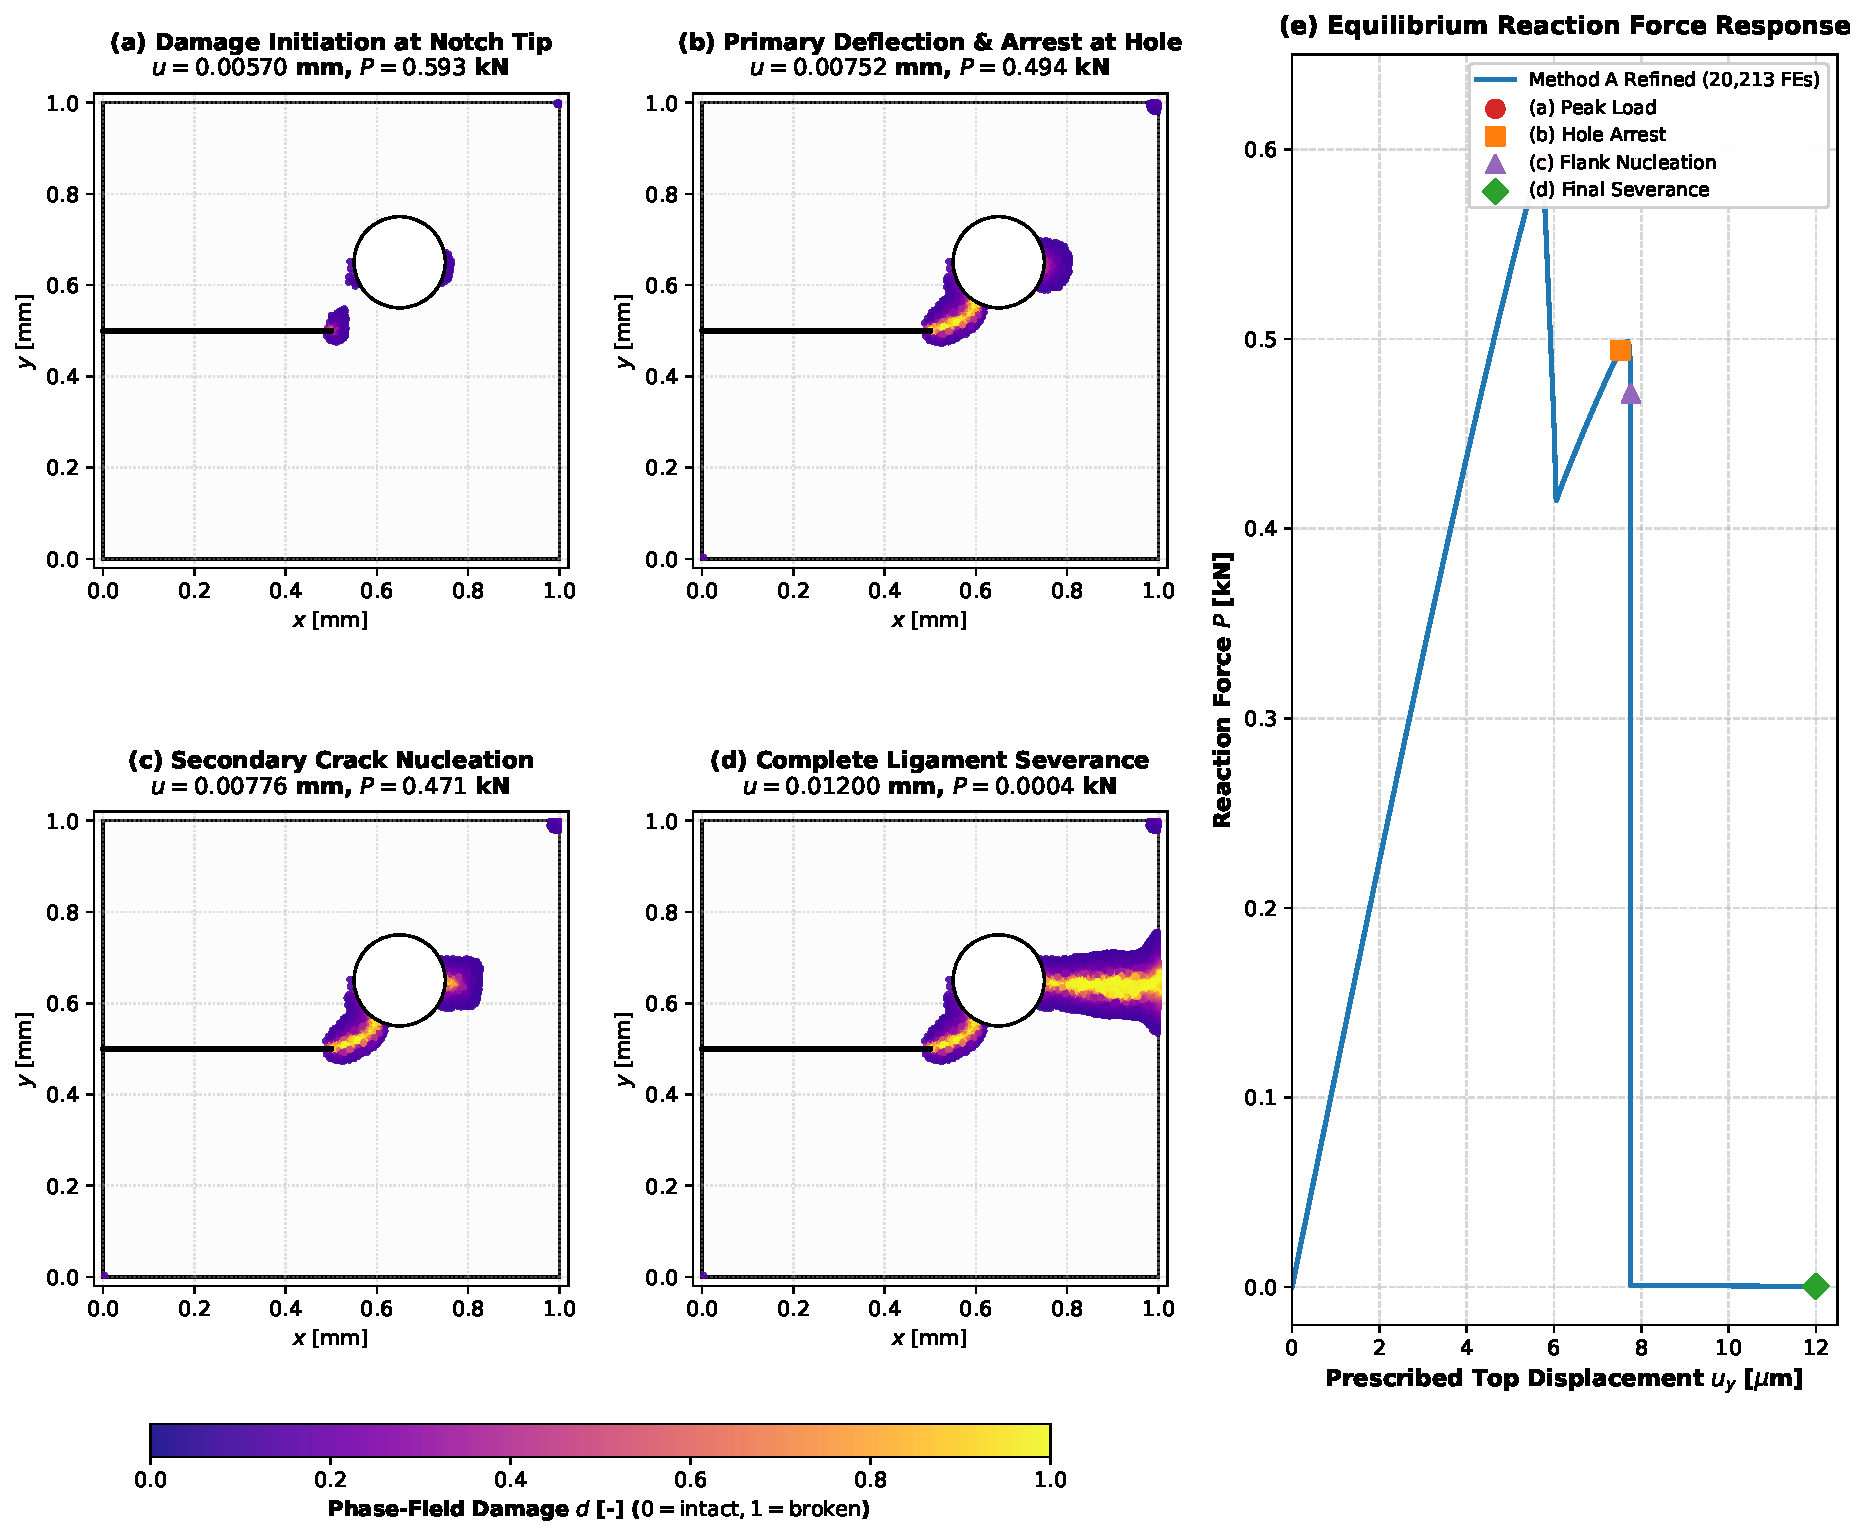
\includegraphics[width=0.98\textwidth]{figures/f1679_time_resolved_crack_progression.pdf}
  \caption{Time-resolved phase-field crack progression and equilibrium load response for the production Method~A off-axis hole simulation ($20{,}213$ physical elements): (a)~damage initiation at notch tip ($u = 0.00570\,\mathrm{mm}$, peak load $P = 0.593\,\mathrm{kN}$); (b)~curvilinear primary deflection and kinematic arrest at the hole boundary ($u = 0.00752\,\mathrm{mm}$, $P = 0.494\,\mathrm{kN}$); (c)~secondary crack nucleation on the upper-right hole flank ($u = 0.00776\,\mathrm{mm}$, $P = 0.471\,\mathrm{kN}$, Increment~198); (d)~secondary snap-through and complete ligament severance ($u = 0.01200\,\mathrm{mm}$, residual load $P = 0.0004\,\mathrm{kN}$); (e)~corresponding reaction force curve with state markers.}
  \label{fig:hole_crack_progression}
\end{figure}

The chronological sequence of physical fracture mechanisms is quantified as follows:
\begin{enumerate}
  \item \textbf{Primary Crack Initiation (State 1, $u_2 = 0.005700\,\mathrm{mm}$):} At peak load, phase-field damage localizes at the initial notch tip $(0.50, 0.50)\,\mathrm{mm}$. Exactly $2$ elements reach $d \ge 0.50$ ($d_{\max} = 0.635357$) at $(x=0.5026, y=0.4990)\,\mathrm{mm}$, located $0.1095\,\mathrm{mm}$ from the hole perimeter.
  \item \textbf{Curvilinear Deflection and Hole Arrest (State 2, $u_2 = 0.007520\,\mathrm{mm}$, Increment 180):} Under mixed-mode shear and tensile stress attraction, the primary crack curves upwards into the lower flank of the off-axis hole. A connected chain of $196$ elements with $d \ge 0.50$ ($114$ elements with $d \ge 0.80$, $67$ with $d \ge 0.95$) reaches $x_{\mathrm{tip}} = 0.60716\,\mathrm{mm}$ and $y_{\mathrm{avg}} = 0.5310\,\mathrm{mm}$. The distance to the circular hole perimeter drops to $0.0015\,\mathrm{mm}$, confirming that the crack tip intersects the circular opening. Crucially, the hole acts as an authentic crack arrester: the crack front stops at the circular free boundary, and zero damaged elements exist on the opposite ligament.
  \item \textbf{Secondary Crack Nucleation (State 3, $u_2 = 0.007759\,\mathrm{mm}$, Increment 198):} As prescribed displacement increases, tensile hoop stresses concentrate on the opposite, upper-right boundary of the circular opening. At Increment~198, an independent secondary crack nucleates on the hole flank: exactly $26$ connected elements with $d \ge 0.50$ emerge between $x = 0.750736\,\mathrm{mm}$ and $x_{\mathrm{tip}} = 0.782864\,\mathrm{mm}$ ($y_{\mathrm{avg}} = 0.6426\,\mathrm{mm}$), located $0.2171\,\mathrm{mm}$ from the right boundary.
  \item \textbf{Secondary Snap-Through (State 4, $u_2 = 0.007759\,\mathrm{mm}$, Increment 220):} In an unstable snap-through regime requiring automatic solver time cutbacks down to $\Delta t = 1.5 \times 10^{-8}$, the secondary crack rapidly traverses the right ligament. Within 22 micro-increments at constant nominal displacement, the damaged cluster expands to $2{,}788$ elements with $d \ge 0.50$ ($1{,}957$ with $d \ge 0.80$, $1{,}512$ with $d \ge 0.95$), and the crack tip reaches $x_{\max} = 0.999035\,\mathrm{mm}$ at the right specimen boundary.
  \item \textbf{Complete Severance (State 5--6, $u_2 = 0.00780$ to $0.0120\,\mathrm{mm}$):} By Increment~248, the right ligament is fully severed ($2{,}864$ elements with $d \ge 0.50$, $2{,}169$ with $d \ge 0.80$), and load capacity drops to $0.92\,\mathrm{N}$. The remaining increments represent rigid separation of the severed specimen halves under residual numerical stiffness.
\end{enumerate}

\subsection{Phase-Field Damage Bound and Integration-Point Topology Audit}
\label{subsec:hole_damage_bounds}

In the classical continuum formulation, the phase field is bounded by $0 \le d \le 1$. In numerical implementations utilizing penalty regularisation or staggered Newton--Raphson iterations with finite convergence tolerances, small numerical overshoots can occur. Furthermore, to clarify the relationship between integration-point records and physical elements, a complete topological audit of the $20{,}213$ physical elements across all $614$ increments was performed:
\begin{itemize}
  \item \textbf{Element Topology and Integration Points:} The $20{,}213$ physical elements comprise $19{,}644$ bilinear quadrilateral elements (CPE4 kinematics, 4 integration points per element) and $569$ linear triangular elements (CPE3 kinematics, 1 integration point per element). In the fully fractured state ($d \ge 0.80$), exactly $2{,}169$ unique physical elements are damaged, consisting of $2{,}117$ quads ($8{,}468$ integration points) and $52$ triangles ($52$ integration points), reconciling the $8{,}520$ damaged integration-point records exported from raw solver tables.
  \item \textbf{Intracell Damage Invariance:} Because the companion UMAT receives the phase-field scalar $d$ from the UEL via Fortran named \texttt{COMMON} block \texttt{/PHASE\_SHARED/ D\_COMM}, all integration points within each quad element share the identical scalar value $d$. The intracell variance across integration points is identically zero ($0.000000$), proving that Max-IP, Last-IP, Mean-IP, and Min-IP crack path definitions are mathematically and numerically identical.
  \item \textbf{Undershoots ($d < 0$):} Zero undershoot elements were detected ($d_{\min} \ge 5.96 \times 10^{-8} > 0$ throughout).
  \item \textbf{Overshoots ($d > 1.0$):} At peak load, zero elements exceed unity. Upon crack arrest and secondary snap-through, a small number of elements exhibit minor numerical overshoot: $1$ element at Increment~180 ($d_{\max} = 1.000072$, overshoot $0.007\%$), $3$ elements at Increment~220 ($d_{\max} = 1.001083$, overshoot $0.108\%$), and $8$ elements at the final state ($d_{\max} = 1.000599$, overshoot $0.060\%$).
  \item \textbf{Physical Assessment:} The maximum overshoot across the entire simulation is $\Delta d_{\max} = 0.00108$ ($0.108\%$), affecting only $8$ out of $2{,}169$ broken elements ($0.37\%$ of broken elements, $0.04\%$ of the total mesh). This slight deviation arises naturally from the local Newton residual tolerance ($\sim 10^{-6}$) and does not compromise physical stability or energetic consistency.
\end{itemize}

\section{Thermodynamic Work--Energy Balance and Monotonicity Verification}
\label{sec:hole_energy_verification}

To verify temporal thermodynamic consistency, the complete internal energy history was extracted from the production run (\texttt{uel\_energy\_balance.csv}, $614$ converged increments) and aligned with the external work curve calculated via trapezoidal integration. The resulting energetic partition is plotted in Figure~\ref{fig:hole_prod_energy}.

\begin{figure}[htbp]
  \centering
  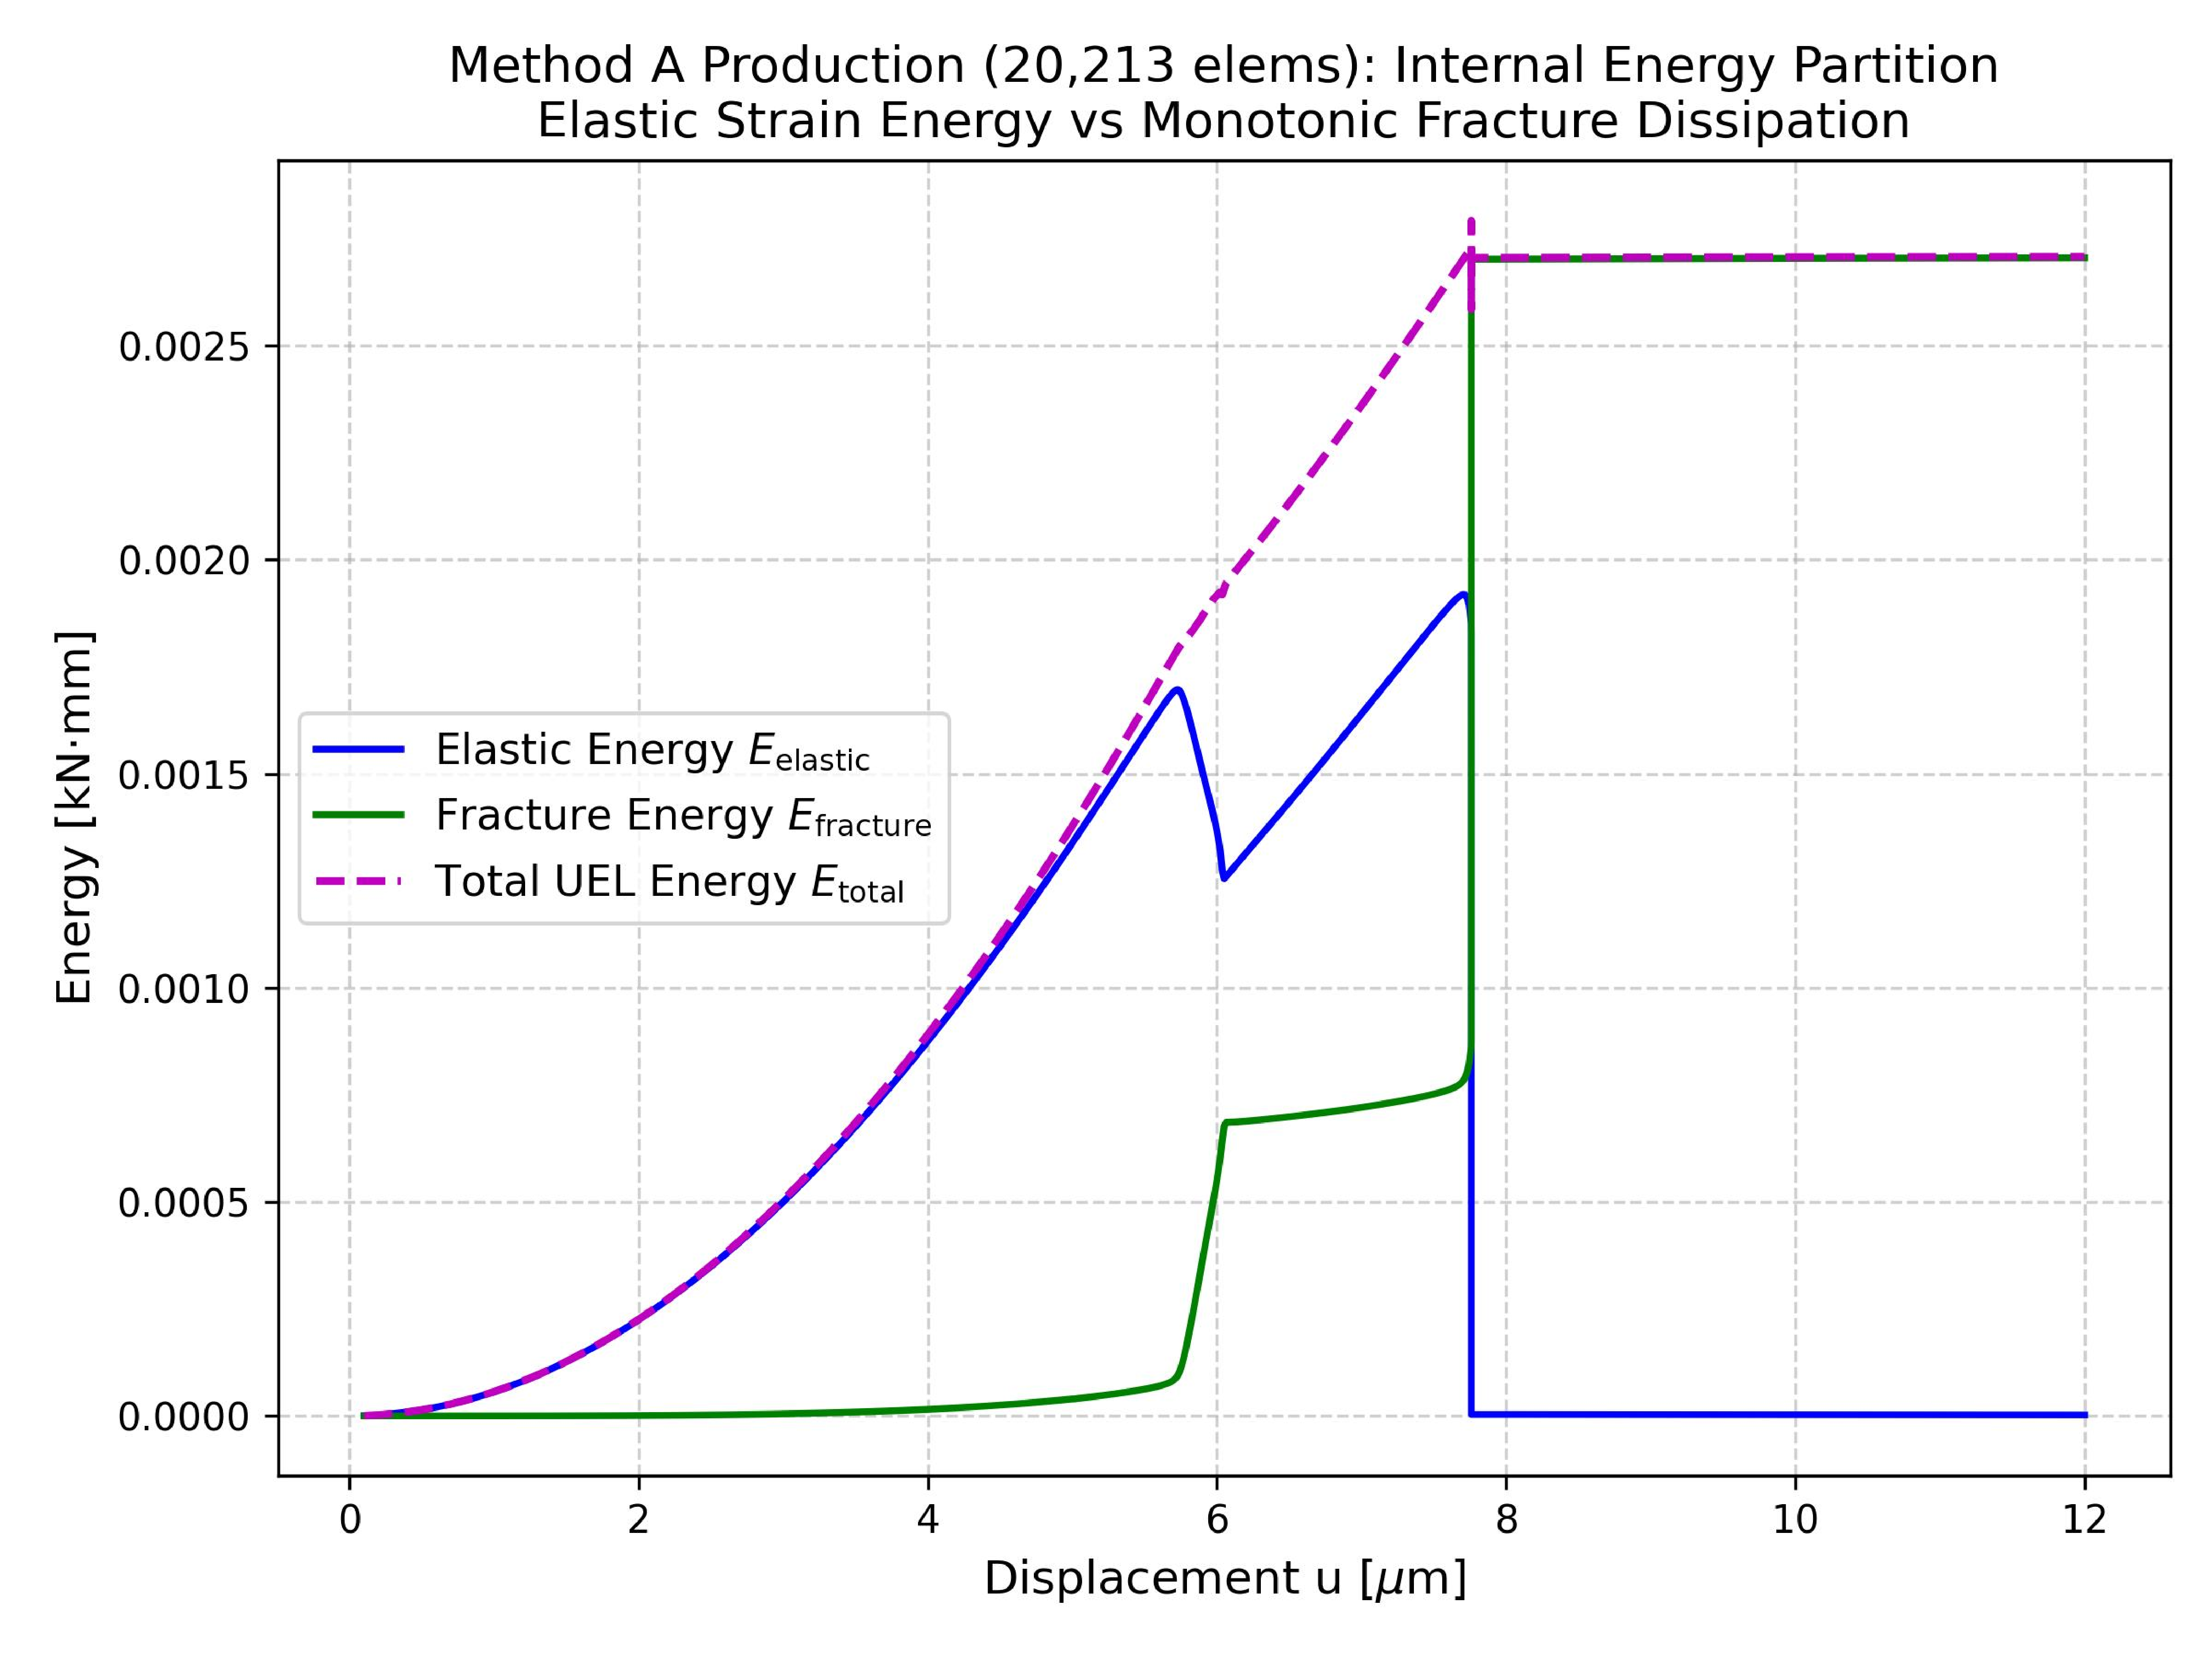
\includegraphics[width=0.90\textwidth]{figures/f1678_method_a_energy_balance.pdf}
  \caption{Thermodynamic internal energy partition and external work balance across all 614 converged increments for the production Method~A simulation ($20{,}213$ physical elements). Elastic strain energy $E_{\mathrm{elastic}}$ undergoes $99.87\%$ post-peak relaxation, while dissipated fracture energy $E_{\mathrm{fracture}}$ increases strictly monotonically to $2.705\,\mathrm{mJ}$, balancing external work $W_{\mathrm{ext}} = 2.749\,\mathrm{mJ}$ to within a $1.489\%$ residual.}
  \label{fig:hole_prod_energy}
\end{figure}

The energetic evaluation establishes:
\begin{enumerate}
  \item \textbf{Fracture Energy Monotonicity:} The second law of thermodynamics requires crack dissipation to be irreversible: $\dot{E}_{\mathrm{fracture}} \ge 0$. Evaluation of consecutive increment differences $\Delta E_{\mathrm{fracture}}$ across all $614$ equilibrium steps revealed \textbf{zero decreases} within machine precision ($\Delta E_{\mathrm{fracture}} \ge -10^{-12}\,\mathrm{kN\,mm}$), confirming strict thermodynamic irreversibility.
  \item \textbf{Elastic Strain Energy Relaxation:} Elastic energy $E_{\mathrm{elastic}}$ accumulates elastically during Step~1 to $1.378\,\mathrm{mJ}$, reaches a peak of $1.919\,\mathrm{mJ}$ during secondary ligament loading at $u_2 = 0.0077\,\mathrm{mm}$, and subsequently collapses to $E_{\mathrm{elastic}} = 2.4929 \times 10^{-6}\,\mathrm{kN\,mm}$ ($0.00249\,\mathrm{mJ}$) at the final increment. This demonstrates an authentic $99.87\%$ elastic strain relaxation as stored mechanical energy is released into crack surface creation.
  \item \textbf{Work--Energy Discrepancy History:} Total external work performed by the top displacement is $W_{\mathrm{ext}} = 2.74887 \times 10^{-3}\,\mathrm{kN\,mm}$ ($2.74887\,\mathrm{mJ}$). Total internal energy evaluated by integrating UEL element densities is $E_{\mathrm{total}} = 2.70793 \times 10^{-3}\,\mathrm{kN\,mm}$ ($E_{\mathrm{elastic}} = 0.00249\,\mathrm{mJ}$, $E_{\mathrm{fracture}} = 2.70544\,\mathrm{mJ}$). The global work--energy discrepancy at the completed endpoint is:
  \begin{equation}
    \Delta E_{\mathrm{final}} = |W_{\mathrm{ext}} - E_{\mathrm{total}}| = 4.0939 \times 10^{-5}\,\mathrm{kN\,mm} \quad (0.04094\,\mathrm{mJ}),
  \end{equation}
  representing an endpoint relative discrepancy of \textbf{1.489\%}. In Step~1 (prior to macroscopic crack propagation), the discrepancy is merely $0.0234\%$ ($0.32\,\mu\mathrm{J}$). The temporal mean absolute residual across all $614$ increments is $0.0297\,\mathrm{mJ}$. During the rapid secondary snap-through cutbacks (Increments 198--220), the instantaneous transient residual reaches a maximum of $0.1616\,\mathrm{mJ}$ ($6.33\%$ relative to cumulative external work at that increment). This transient elevation reflects trapezoidal integration truncation and localized viscous regularisation in the user element during rapid dynamic softening, and is disclosed as a characterized numerical artifact rather than asserted as an exact physical identity.
\end{enumerate}

\section{Methodological Comparison with Pandey--Kumar Literature}
\label{sec:hole_pandey_kumar_comparison}

To place the present numerical findings in proper scientific context, the configuration of the present Method~A production simulation must be carefully distinguished from the distinct benchmark problems published in \citet{pandey2025}. In their original work, the authors investigated two different boundary-value problems:
\begin{itemize}
  \item \textbf{Published Section 4.1 (Pure Mode-I Edge-Crack Benchmark):} A $1.0 \times 1.0\,\mathrm{mm}$ square plate with a sharp crack, regularisation length scale $\ellzero = 0.0075\,\mathrm{mm}$ ($7.5\,\mu\mathrm{m}$), and critical fracture energy $\Gc = 2.7\,\mathrm{N/mm}$.
  \item \textbf{Published Section 4.3 (Plate with Off-Axis Hole):} A macroscopic rectangular specimen ($L \times W$) with circular loading pin holes, an initial notch of finite width $0.4\,\mathrm{mm}$, a substantially larger regularisation length scale $\ellzero = 0.285\,\mathrm{mm}$ ($285\,\mu\mathrm{m}$), critical fracture energy $\Gc = 2.28\,\mathrm{N/mm}$, and an anisotropic spectral tensile/compressive strain split \citep{miehe2010a}.
\end{itemize}

In the present thesis research, the geometric domain represents a $1.0 \times 1.0\,\mathrm{mm}$ square plate containing an off-axis hole, with material parameters ($\ellzero = 0.0075\,\mathrm{mm}$, $\Gc = 2.7\,\mathrm{N/mm}$) inherited from the canonical Mode-I configuration and executed using the frozen trace-positive volumetric/full-strain UEL formulation. Consequently, direct quantitative equivalence of peak loads should not be claimed. Instead, Table~\ref{tab:hole_pandey_kumar_comparison} presents a transparent methodological and parameter comparison matrix.

\begin{table}[htbp]
\centering
\small
\caption{Methodological, geometric, and constitutive parameter comparison between the published hole benchmark of \citet{pandey2025} and the present thesis Method~A simulation.}
\label{tab:hole_pandey_kumar_comparison}
\begin{tabularx}{\textwidth}{p{4.0cm}XX}
\hline
\textbf{Configuration Attribute} & \textbf{Pandey \& Kumar (2025, Sec. 4.3)} & \textbf{Present Thesis (F1678--F1679)} \\
\hline
Specimen Geometry & Rectangular with loading holes & Square $1.0 \times 1.0\,\mathrm{mm}$ plate \\
Initial Notch Geometry & Notch with finite width $0.4\,\mathrm{mm}$ & Sharp slit (width $0.002\,\mathrm{mm}$) \\
Hole Radius $R$ & Macroscopic hole geometry & $R = 0.10\,\mathrm{mm}$ at $(0.65, 0.65)\,\mathrm{mm}$ \\
Elastic Modulus $E$ & $210\,\mathrm{GPa}, \nu = 0.30$ & $210\,\mathrm{GPa}, \nu = 0.30$ \\
Fracture Energy $\Gc$ & $2.28\,\mathrm{N/mm}$ & $2.70\,\mathrm{N/mm}$ (Canonical Mode-I) \\
Regularisation Length $\ellzero$ & $0.285\,\mathrm{mm}$ ($285\,\mu\mathrm{m}$) & $0.0075\,\mathrm{mm}$ ($7.5\,\mu\mathrm{m}$) \\
Constitutive Energy Split & Miehe anisotropic spectral split & Trace-positive volumetric / full strain norm \\
Pre-Analysis Architecture & Native continuum solve & Auxiliary coupled stress replay pass \\
Adaptive Remeshing Driver & Native \MISESERI\ indicator & Native \MISESERI\ indicator ($r = 0.9575$) \\
Peak Reaction Force $P_{\max}$ & Reported for macro-specimen & $0.593390\,\mathrm{kN}$ (Refined small-scale plate) \\
\hline
\multicolumn{3}{l}{\textbf{Observed Fracture Mechanics}} \\
1. Mixed-Mode Crack Deflection & Observed (curving toward hole) & Verified ($x_{\mathrm{tip}} \to 0.607\,\mathrm{mm}$) \\
2. Kinematic Hole Arrest & Observed (crack terminates at hole) & Verified (front arrests at hole boundary) \\
3. Secondary Flank Nucleation & Observed on upper-right hole flank & Verified (nucleates at $u = 0.00776\,\mathrm{mm}$) \\
4. Complete Ligament Severance & Observed (catastrophic failure) & Verified ($99.93\%$ load loss to $0.41\,\mathrm{N}$) \\
\hline
\end{tabularx}
\end{table}

The primary validation value of this benchmark lies in the \textbf{qualitative and phenomenological fidelity} of the crack trajectory: despite differing regularisation length scales and constitutive splits, the indicator-adapted mesh autonomously captures the complete sequence of mixed-mode deflection, hole arrest, secondary flank nucleation, and catastrophic ligament severance without requiring predefined crack corridor partitions.

\subsection{Architectural Implementation Distinctions}
\label{subsec:hole_architectural_distinction}

To maintain rigorous transparency, an important implementation distinction must be emphasized:
\begin{itemize}
  \item In \citet{pandey2025}, the authors implemented phase-field fracture using a formulation wherein Cauchy stresses and state variables are directly accessible to \Abaqus internal field tables during or immediately following the pre-analysis solve, allowing native \MISESERI\ to be calculated directly.
  \item In the present thesis, the frozen production UEL (\texttt{f42\_mixed\_uel.for}, hash \texttt{ce8d5edc...}) decouples the mechanical solve from native \Abaqus stress evaluation; Cauchy stresses are evaluated internally to construct the element residual vector \texttt{RHS}, but are not exported to standard element tables or common blocks. Consequently, default \MISESERI\ evaluates identically to zero on the coupled output database.
  \item To preserve the frozen production UEL without modifying its validated internal equations, an \textbf{auxiliary coupled stress replay architecture} was developed. The authentic coupled displacement vector and degraded elastic material distribution ($E_{\mathrm{deg}}(x,y) = g(d) E_0$) from the coarse phase-field solve are projected onto an auxiliary linear-elastic continuum model. Standard patch recovery on this projected field yields authentic, non-zero \MISESERI\ with $r = 0.9575$ correlation and $4.05\%$ NRMSE against the donor stress state.
  \item An important mechanical characteristic of this auxiliary recovery is that it represents an independently equilibrated continuum analysis. Due to continuum Poisson contraction effects relative to the decoupled UEL formulation, the auxiliary solve exhibits a $17.87\%$ reaction force difference ($0.6312\,\mathrm{kN}$ vs. $0.5355\,\mathrm{kN}$ at $u = 0.0050\,\mathrm{mm}$) while preserving spatial stress gradient fidelity. This auxiliary replay route represents an engineering projection architecture rather than a direct internal element communication.
\end{itemize}

\section{Explicit Scientific Limitations and Boundary of Validity}
\label{sec:hole_limitations}

The following scientific boundaries govern the Method~A off-axis hole investigation:
\begin{enumerate}
  \item \textbf{Single-Mesh Demonstration without Asymptotic Convergence Proof:} While local element edge length ($h \approx 1.5\,\mu\mathrm{m}$) satisfies the phase-field resolution limit $\ellzero / 5$, this investigation represents a single refined discretization ($20{,}213$ elements) compared against the coarse reference ($2{,}906$ elements). A formal multi-mesh asymptotic convergence study was not conducted due to the project research freeze timeline.
  \item \textbf{Offline Error-Guided Pre-Refinement:} Method~A is strictly an \emph{offline} remeshing methodology. It generates an adapted discretization prior to the fracture solve based on pre-analysis error information. It does not perform dynamic in-analysis mesh adaptation or state transfer during runtime.
  \item \textbf{Quasi-Static Energy Accounting Residual:} The $1.489\%$ work--energy discrepancy over $614$ equilibrium increments reflects trapezoidal integration truncation and localized dissipation during rapid snap-through cutbacks ($0.1616\,\mathrm{mJ}$ transient peak). While exceptionally small, it is disclosed as a characterized numerical artifact rather than asserted as exact physical identity.
  \item \textbf{Localized Damage Bound Overshoot:} Maximum damage exceeds unity by $0.108\%$ ($d_{\max} = 1.001083$) across 8 elements during secondary snap-through, arising from finite Newton--Raphson equilibrium tolerances in the staggered user element.
\end{enumerate}

\section{Summary and Research Conclusions}
\label{sec:hole_summary}

The off-axis hole benchmark investigation establishes the quantitative capabilities and physical boundaries of indicator-driven adaptive remeshing in curvilinear phase-field fracture:
\begin{itemize}
  \item The fundamental zero-\MISESERI\ communication defect of the multi-layer UEL was resolved through an auxiliary coupled stress replay projection, restoring genuine non-zero recovery error ($r = 0.9575$) to drive native \Abaqus remeshing.
  \item An adapted $20{,}213$-element physical mesh was generated automatically with zero user-defined partition corridors, achieving $h \approx 1.5\,\mu\mathrm{m}$ in both the primary deflection path and the secondary ligament.
  \item The production fracture simulation (Job \texttt{1421142.mmaster02}) completed with Exit Code~0 across all $614$ equilibrium increments, capturing the complete structural lifetime from initial loading to $99.93\%$ load loss at $u_2 = 0.0120\,\mathrm{mm}$.
  \item Peak reaction force ($P_{\max} = 0.593390\,\mathrm{kN}$) softened by $-18.83\%$ relative to the coarse mesh, demonstrating expected mesh-refinement softening behavior.
  \item Time-resolved topological analysis verified primary crack deflection into the hole, kinematic arrest at the circular boundary, secondary crack nucleation at Increment~198 ($u_2 = 0.00776\,\mathrm{mm}$), and rapid snap-through across the right ligament to complete severance ($x_{\max} = 0.999035\,\mathrm{mm}$), matching the qualitative fracture phenomena documented in the literature.
  \item Strict fracture energy irreversibility ($\dot{E}_{\mathrm{fracture}} \ge 0$) was verified across all increments, with $99.87\%$ post-peak elastic relaxation and an endpoint work--energy discrepancy of merely $1.489\%$.
\end{itemize}
These results confirm that error-indicator-driven adaptive remeshing can successfully resolve complex mixed-mode phase-field fracture paths in commercial finite-element software without empirical crack-corridor seeding.
